\documentclass[lang=cn,math=cm,chinesefont=nofont,11pt,scheme=chinese,onecol]{elegantbook}
\setCJKmainfont[BoldFont={FZHei-B01},ItalicFont={FZKai-Z03}]{FZShuSong-Z01}
\setCJKsansfont{FZHei-B01}
\setCJKfamilyfont{zhsong}{FZShuSong-Z01}
\setCJKfamilyfont{zhhei}{FZHei-B01}
\setCJKfamilyfont{zhkai}{FZKai-Z03}
\setCJKfamilyfont{zhfs}{FZFangSong-Z02}
\setCJKfamilyfont{zhli}{FZLiShu-S01}

\newcommand*{\songti}{\CJKfamily{zhsong}} % 宋体
\newcommand*{\heiti}{\CJKfamily{zhhei}} % 黑体
\newcommand*{\kaiti}{\CJKfamily{zhkai}} % 楷体
\newcommand*{\fangsong}{\CJKfamily{zhfs}} % 仿宋
\newcommand*{\lishu}{\CJKfamily{zhli}}    % 隶书
\linespread{1.3}

\usepackage{graphicx}
\usepackage{amssymb}
\usepackage{epigraph}
\usepackage{setspace}

\title{数学之桥:从初等数学到微积分}
\subtitle{Powered by \LaTeX.}

\author{Siliconet}
\date{始于2023年}
\version{0.1}
\bioinfo{模板}{ElegantBook}

\extrainfo{你站在桥上看风景,看风景人在楼上看你。明月装饰了你的窗子,你装饰了别人的梦。}

\setcounter{tocdepth}{3}

\cover{cover.jpg}

% 本文档命令
\usepackage{array}
\newcommand{\ccr}[1]{\makecell{{\color{#1}\rule{1cm}{1cm}}}}

% 修改标题页的橙色带
\definecolor{customcolor}{RGB}{255,255,255}
\colorlet{coverlinecolor}{customcolor}
\usepackage{cprotect}

\addbibresource[location=local]{reference.bib} % 参考文献,不要删除

\setcounter{tocdepth}{1}
%设置目录显示深度

\begin{document}

\maketitle
\frontmatter

\tableofcontents

\mainmatter

\chapter{集合论初步}

本项目采用ElegantBook作为模板,模板地址:

GitHub:\href{https://github.com/ElegantLaTeX/ElegantBook}{https://github.com/ElegantLaTeX/ElegantBook}

CTAN:\href{https://ctan.org/pkg/elegantbook}{https://ctan.org/pkg/elegantbook}

本书的GitHub开源地址:

\href{https://github.com/Siliconet/Math-Bridge}{https://github.com/Siliconet/Math-Bridge}

\section{集合的概念与表示}
集合论是学习数学的基础。基础到什么地步呢?集合论在几乎所有其他数学分支领域中都是基础内容。一方面,它作为一种表示工具存在。集合可以用来表示各种东西,比如说奇数、偶数、质数、合数。另一方面,集合是逻辑推理的基础,这意味着要继续学习接下来的内容,先学集合是必不可少的。(没错下一章就是简易逻辑,虽然集合论远不止于此)

那为什么不从小学开始学呢?普通小学生一开始学不懂嘛。

\subsection{集合的概念}

我们先给出对于集合这个概念的一个比较抽象的描述:\textbf{集合}(简称\textbf{集})是一些具有某种特定性质的对象组成的总体。

怎么理解这个特定性质呢?比如说,身高高于165cm算不算一个特定性质?显然算嘛。所以我们可以这么说:“我的班上身高高于165cm的同学”能构成一个集合。

满足某个特定的不等式算不算特定性质?算。于是解集(你在初中已经见过)这个概念诞生了,就是解的集合。

我们研究的很多东西都可以构成集合。构成集合的对象可以是各种事物,可以是物,也可以是人,可以是数,也可以是图形,甚至可以是集合(没错就是套娃)……构成集合的对象称为这个集合的\textbf{元素}。

比方说,以2023年《财富》世界500强排行榜当中的前5名作为一个集合,那么这个集合的元素是:沃尔玛、沙特阿美公司、国家电网有限公司、亚马逊、中国石油天然气集团有限公司。

现在,我们来谈谈集合的分类。按照集合中含有的元素的个数,我们把集合分成两类:\textbf{有限集}(含有有限个元素的集合)和\textbf{无限集}(含有无限个元素的集合)。

这里还要提到两种特别的集合:

\textbf{空集}(记作$\varnothing$)是不含任何元素的集合;\textbf{单元素集}是只含一个元素的集合。

\hspace*{\fill}

我们通常用英文大写字母$A$,$B$,$C$,$\cdots$表示集合,用小写英文字母$a$,$b$,$c$,$\cdots$表示集合的元素。

如果$a$是集合$A$的元素,我们就记作$a\in A$,读作“$a$属于$A$”,与此相反的情况是,如果$a$不是集合$A$的元素,我们就记作$a\notin A$,读作“$a$不属于$A$”。

那么问题来了,$\varnothing \in \{\varnothing\}$是不是正确的?是。因为$\varnothing$是$\{\varnothing\}$当中的一个元素,二者并不相同。

\subsection{集合的特性}

\begin{itemize}
  \item 确定性:集合中的每一个元素都是确定的。比如说,“我的班上身高比较高的同学”不能构成一个集合。倘若有人发问:身高180cm算不算高?身高160cm算不算高?这就不好回答了。没有一个明确的标准是无法确定身高到底算不算“比较高”的。我们现在把它修改为“我的班上身高大于等于175cm的同学”,这样就可以构成一个集合。
  
  \item 无序性:集合中的元素没有确定的顺序。也就是说,集合$\left\{a,b,c \right\}$和集合$\left\{b,a,c \right\}$是同一个集合。
\end{itemize}

按照Thomas J. Jech的《Set Theory》及知乎“無雙”的文章(链接:\href{https://zhuanlan.zhihu.com/p/713264884}{https://zhuanlan.zhihu.com/p/713264884})当中的说法,用列举法表示集合时,集合中的元素可以重复出现,但在计算元素数量时,相同的元素只能算为一个。用列举法时若出现相同的元素,只写一个即可。

但是,现行的高中数学教材(2024.8.10)均认为集合的元素是互不相同的。

\subsection{常用的数集}
现在来看几个比较常用的数集:

1.所有非负整数构成的集合称为\textbf{自然数集},记作$\mathbb{N}$。友情提示,$0\in \mathbb{N}$。

2.所有正整数构成的集合称为\textbf{正整数集},记作$\mathbb{N}_+$或者$\mathbb{N}^*$。

3.所有整数构成的集合称为\textbf{整数集},记作$\mathbb{Z}$。

4.所有有理数构成的集合称为\textbf{有理数集},记作$\mathbb{Q}$。

5.所有实数构成的集合称为\textbf{实数集},记作$\mathbb{R}$。

还有一些比较特别(用得比较少)的数集,如正有理数集$\mathbb{Q}^+$,负实数集$\mathbb{R}^-$,正实数集$\mathbb{R}^+$。

此外,由点组成的集合称为\textbf{点集}。

\subsection{集合的表示}
集合有两种主要的的表示方法:\textbf{列举法}和\textbf{描述法}。

把集合里的元素全部列出来,写在花括号内,并且元素之间用逗号分隔,这种表示集合的方法称为\textbf{列举法}。

举三个例子:

\begin{example}
  12的所有因数组成的集合可以表示为$\{-12,-6,-4,-3,-2,-1,1,2,3,4,6,12\}$.
\end{example}
\begin{example}
  唐宋八大家的姓名组成的集合可以表示为$\{\text{韩愈,柳宗元,欧阳修,苏洵,苏辙,苏轼,王安石,曾巩}\}$。
\end{example}
\begin{example}
  用集合重新定义圆:
\end{example}
\begin{definition}[圆]
  圆是平面内与一个定点距离为定长的点的集合。
\end{definition}
这里我们只是用集合把初中学过的圆的定义重新描述了一遍。

如果一个集合的元素很多,我们可以列举几个元素表示元素的规律,其余的用省略号代替。

\begin{example}
  自然数集可以这么表示:$\{0,1,2,\cdots,n,\cdots\}$。
\end{example}

对于元素个数有限的集合,我们要把最后一个元素给写出来。
\begin{example}
  小于或等于50的自然数组成的集合可以这么表示:$\{0,1,2,\cdots,50\}$。
\end{example}


列举法当然是不能解决全部集合的表示问题的,比方说,不等式$2x\geq 0$的解集怎么用列举法表示?这时候我们就需要\textbf{描述法}了。

先举个例子。以上面这个不等式为例,满足$x\geq 0$的实数都是这个不等式解集的元素,而不满足$x\geq 0$的实数都不是。所以我们可以这么表示该解集:
$$\{x\mid x\geq0\}$$

\begin{definition}[特征性质]
如果属于集合$a$的任意一个元素$x$都具有性质$p(x)$,而不属于集合$A$的元素都不具有这个性质,则称性质$p(x)$为集合$A$的一个\underline{特征性质}。一个集合可以有多个特征性质。
\end{definition}
比方说,上面的$x\geq 0$就是上面的不等式解集的特征性质。

于是我们就可以用特征性质来表示集合:$$\{x\mid p(x)\}$$

这就是\textbf{描述法},全称是\textbf{特征性质描述法}。

\begin{example}
  所有4的倍数组成的集合为$\{x\mid x=4n,n\in\mathbb{Z}\}$。当然写成$\{\text{4的倍数}\}$也没问题。
\end{example}

\begin{example}
  不等式$2x-7\geq 0$的解集可表示为$\{x\mid x\geq\frac{7}{2}\}$,也可以直接表示成$\{x\mid 2x-7\geq 0\}$。这里我们推荐前者,因为是化简过的。
\end{example}

\begin{example}
  平面直角坐标系内第一象限的所有点组成的集合为$\{(x,y)\mid x>0,y>0\}$。把逗号换为“且”也是可以的。
\end{example}

\begin{example}
  所有的正奇数组成的集合为$\{x\mid x=2n+1,n\in\mathbb{N}\}$,也可以写成$\{x\in\mathbb{N}\mid x=2n+1,n\in\mathbb{Z}\}$,二者是一样的。
\end{example}

\begin{remark}
  对于一个集合$\{x\mid p(x)\}$,它当中所有属于另一个集合$\boldmath{I}$(我们默认研究实数范围内的数,所以$\boldmath{I}$为$\mathbb{R}$时通常省略)的元素组成的集合,可以表示为$$\{x\in\boldmath{I}\mid p(x)\}$$
\end{remark}

\begin{example}
  \label{exp:1}
  所有的奇数组成的集合为$\{x\mid x=2n+1,n\in\mathbb{Z}\}$,也可以写成$\{x\in\mathbb{Z}\mid x=2n+1,n\in\mathbb{Z}\}$,二者是一样的。奇数集还可以表示为$\{x\mid x=2n-1,n\in\mathbb{Z}\}$,甚至是$\{x\mid x=2n-3,n\in\mathbb{Z}\}$(你可以使用列举法验证这个说法的正确性),当然我们更多地使用第1、3两种。
\end{example}

如果不会引起混淆的话,竖线及其左边的部分可以省略。如所有锐角三角形构成的集合可表示为$\{\text{锐角三角形}\}$。

\subsection{区间}
当我们用不等号表示数的范围时,我们一般不会觉得繁琐。但是,当这个范围分成几段时,就容易显得麻烦。比方说,不等式$x^4-19x^3+110x^2-197x+69>0$(这个不等式的解法我们目前还没学,但是不影响接下来的学习)的解集为$x<\dfrac{1}{2} \left(7-\sqrt{37}\right)\text{或}6-\sqrt{13}<x<\dfrac{1}{2} \left(\sqrt{37}+7\right)\text{或}x>\sqrt{13}+6$,有点麻烦。

怎样把这个表达化简一下呢?

我们可以使用区间来表达。

\begin{definition}[区间]
	设$a,b\in\mathbb{R}$,且$a<b$,则\\集合$\{x\mid a\leq x\leq b\}$可简写为$[a,b]$,称为\underline{闭区间};\\集合$\{x\mid a<x<b\}$可简写为$(a,b)$,称为\underline{开区间};\\集合$\{x\mid a\leq x<b\}$可简写为$[a,b)$,称为\underline{左闭右开区间};集合$\{x\mid a< x\leq b\}$可简写为$(a,b]$,称为\underline{左开右闭区间},合称\underline{半开半闭区间}。
\end{definition}

这样还不够,我们还需要用区间表示诸如“$\left\{x\mid x>0\right\}$”一类的集合。因此我们还需要定义无穷区间。

\begin{definition}[无穷区间]
    设$a\in\mathbb{R}$,则集合$\{x\mid x\geq a\}$可简写为$[a,+\infty)$,集合$\{x\mid x>a\}$可简写为$(a,+\infty)$,集合$\{x\mid x\leq a\}$可简写为$(-\infty,a]$,集合$\{x\mid x<a\}$可简写为$(-\infty,a)$。
\end{definition}

那么,上面的不等式的解集就可以表示为$(-\infty,\dfrac{1}{2} \left(7-\sqrt{37}\right))\cup (6-\sqrt{13},\dfrac{1}{2} \left(\sqrt{37}+7\right))\cup (\sqrt{13}+6,+\infty)$,虽然也比较长,但是相比之前的还是要简短一点。

\begin{example}
  不等式$\begin{cases}3x-(x-3)\geqslant1\\\dfrac{2x+1}{3}>x-1\end{cases}$的解集为$[-1,4)$。
\end{example}

\begin{example}
  使式子$\sqrt{2x-3}$有意义的所有实数组成的集合为$[\dfrac{3}{2},+\infty)$。
\end{example}

\subsection{习题}

\begin{exercise}\label{exer:1}
  用符号“$\in$”或“$\notin$”填空:\\
(1)$1\_\_\_\mathbb{N}$;(2)$0\_\_\_\varnothing$;(3)$(2,7)\_\_\_\{(x,y)\mid x+2y=3\}$;(4)$-1\_\_\_\{x\mid x^{3}<2\}$;\\(5)$2024\_\_\_\{x\mid x=4n-1,n\in\mathbb{Z}\}$.
\end{exercise}

\begin{exercise}\label{exer:2}
  下列集合是有限集还是无限集?\\
  (1)$\{\text{周长等于20cm的三角形}\}$;(2)$\{\text{太阳系八大行星}\}$;(3)$\{\text{大于10的素数}\}$.
\end{exercise}

\begin{exercise}\label{exer:3}
  用列举法表示下列集合:\\
  (1)$\{x\mid x^2+2=6\}$;
  (2)绝对值小于3的所有整数组成的集合;
  (3)能整除所有自然数的数组成的集合。
\end{exercise}

\begin{exercise}\label{exer:4}
  用描述法表示下列集合:\\
  (1)平面直角坐标系第一象限内所有点的坐标;
  (2)所有矩形组成的集合;
  (3)$\{1,5,25,125,625\}$.
\end{exercise}

\begin{exercise}\label{exer:5}
  写出方程组$\left.\left\{\begin{aligned}x+y&=3\\y+z&=4\\z+x&=5\end{aligned}\right.\right.$的解集。
\end{exercise}

\begin{exercise}\label{exer:6}
  已知集合$A=\{x-2,x+5,12\}$,且$-3\in A$,求$x$的值。
\end{exercise}

\begin{exercise}\label{exer:7}
  设$P$表示平面$a$内的动点,$A,B,O$分别是平面$\alpha$内的三个定点,属于下列集合的点构成平面$\alpha$内的什么图形?\\
  (1)$\{P||PA|=|PB|\}$;
  (2)$\{P||PO|=3\text{cm}\}$
  (3)$\{P||PO|\geqslant2\text{,且}|PO|\leqslant3\}$
\end{exercise}

\begin{exercise}\label{exer:8}
  简化下列集合的表达:\\
  (1)$\{y\mid y=x^2,x\in\mathbb{R}\}$;
  (2)$\{y\mid y=\dfrac{1}{x},x\in\mathbb{R}\text{,且}x\neq0\}$;
  (3)$\{(x,y)\mid x=0\text{,}y\in R\}$.
\end{exercise}

\begin{exercise}\label{exer:9}
  已知集合$A=\{x\mid(m-1)x^2-2x+1=0\}$中至多含有一个元素,求实数$m$的取值范围.
\end{exercise}
\begin{remark}
  以后如无特殊说明,解集、取值范围等一律用集合表示。
\end{remark}

\begin{exercise}\label{exer:202406261951}
  对于集合$\{x\mid a\leq x\leq b\}$,我们把$b-a$称为它的长度。设集合$A=\{x\mid a\leq x\leq a+1981\},B=\{x\mid b-1014\leq x\leq b\}$,且$A,B$都是集合$U=\{x\mid 0\leq x\leq 2012\}$的子集,则集合$A\cap B$的长度的最小值是\underline{\hbox to 25mm{}}.
\end{exercise}

\section{集合的关系与运算}
从本节开始,证明性的内容会逐渐增加,当然难度也上来了。
\subsection{子集}
先来看一个例子:$$A=\{1,2,3,4,5\}\;B=\{1,2,3,4,5,6,7\}$$
显然,$A$中的任意一个元素都在$B$中。
类似这样地,我们给出子集的定义:
\begin{definition}[子集]
  如果集合$A$的任意一个元素都是集合$B$的元素,那么集合 A 称为集合$B$的子集,记作$A\subseteq B$或$A\subset B$或$B\supseteq A$。前两个读作“$A$包含于$B$”,后一个读作“$B$包含$A$”。

  如果$A$不是$B$的子集,记作$A\nsubseteq B$或$B\nsupseteq A$,读作“$A$不包含于$B$”或“$B$不包含$A$”。
\end{definition}
不同的人符号习惯可能不同,多见几种表示方法也不是不可以(前提是不弄乱)如同鲁迅的《孔乙己》当中:
\begin{quotation}
  “对呀对呀!……回字有四样写法,你知道么?”——《孔乙己》
\end{quotation}

根据定义便可以得到:$\mathbb{N}\subseteq\mathbb{Z}\subseteq\mathbb{Q}\subseteq\mathbb{R}$.

  另外,集合有一个基本的性质:
\begin{property}
  任何集合都是其本身的子集。
\end{property}

另外,我们规定,空集是任意集合的子集。做题时请格外注意这一点。

\begin{example}
  写出集合$\{a,b,c\}$的所有子集。
\end{example}
\begin{remark}
  建议在写子集时按元素个数从小到大写,并且不要忽略空集。
\end{remark}
\begin{solution}
  集合$\{a,b,c\}$的所有子集为$\varnothing ,\{a\},\{b\},\{c\},\{a,b\},\{a,c\}\{b,c\},\{a,b,c\}$.
\end{solution}
\begin{definition}[集合的相等]
  对于集合$A$、$B$,如果有$A\subseteq B$,且$B\subseteq A$,则称集合$A$和$B$\underline{相等},记作$A=B$。
\end{definition}

在下面的例子中,你将看到一组特殊的相等集合。

\begin{example}\label{exp:2}
  判断下列两个集合是否相等。
  $$A=\left\{n\mid n=4k\pm1,k\in\mathbf{Z}\right\};B=\left\{m\mid m=2k+1,k\in\mathbf{Z}\right\}$$
\end{example}
\begin{solution}
  我们根据定义来证明(以后的相当一部分命题证明都是如此)。

一方面,集合$B$是奇数集(我们在1.1的例\ref{exp:1}中提到),而集合$A$的所有元素都是奇数,所以$A\subseteq B$。

另一方面,奇数$m$除以4的余数只可能是1或3(如果余数是0或2,$m$就是偶数了),如果余数为1,那么$m=4k+1(k\in\mathbb{Z})$,因此$m\in A$;如果余数为3,那么$m=4k+3=4(k+1)-1(k\in\mathbb{Z})$,$m\in A$同样成立。所以$B\subseteq A$。

综上,$A=B$。
\end{solution}

下面来看看真子集。
\begin{definition}[真子集]
  对于集合$A$、$B$,如果 $A\subseteq B$,并且$B$中至少有一个元素不属于$A$,那么集合$A$叫做集合$B$的真子集,记作$A\subsetneqq B$或$B\supsetneqq A$,读作“$A$真包含于$B$或$B$真包含$A$”。
\end{definition}

\begin{example}
  写出集合$\{a,b,c\}$的所有真子集。
\end{example}
\begin{solution}集合$\{a,b,c\}$的所有真子集为$\varnothing ,\{a\},\{b\},\{c\},\{a,b\},\{a,c\}\{b,c\}$.
\end{solution}

\begin{remark}
  你可以与本节例1比较一下。
\end{remark}

\subsection{Venn图}
  \underline{Venn图}(或者说\underline{韦恩图})是一种用图形直观表示集合关系的方法。图像当然比文字更为直观,所以在解决某些问题时可以借助Venn图理清集合的关系。

\begin{example}
  用Venn图表示集合$A\subseteq B$.
\end{example}
\begin{solution}
  如图\ref{img:Venn1}所示。
\end{solution}
\begin{figure}[h]
  \centering
  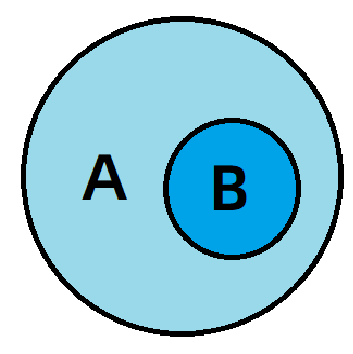
\includegraphics[width=0.1\textwidth]{image/Venn1.png}
  \caption{Venn图示例}
  \label{img:Venn1}
\end{figure}

\subsection{全集与补集}
  我们研究集合间的关系时,这些集合可能都是某一个给定的集合的子集,我们称这个给定的集合为\underline{全集}。我们一般记全集为$U$。比如说,解不等式时,我们默认全集为$\mathbb{R}$。

  接下来是补集。
\begin{definition}{补集}
  设全集为$U$,集合$A\subseteq U$,由$U$中所有不属于$A$的元素组成的集合称为$A$在$U$中的\underline{补集},记作${\complement}_{U}A$(若不会产生歧义,即只有一个全集的情况下,也可以记作$\overline{A}$或者$A^c$).读作“$A$在$U$中的补集”。即

  $${\complement}_{U}A=\{x|x\in I\text{,且}x\notin A\}.$$
\end{definition}
\begin{remark}
  此后如无特殊说明,我们默认$U$为全集。由于不同人的符号习惯不同,你可能会在一些地方见到用“$I$”表示全集的。
\end{remark}
  然后来看几个例子。
\begin{example}
  $\complement_{U}A$用Venn图表示如图\ref{img:Venn3}所示,上色部分即为$\complement_{U}A$.
\end{example}
\begin{figure}[h]
  \centering
  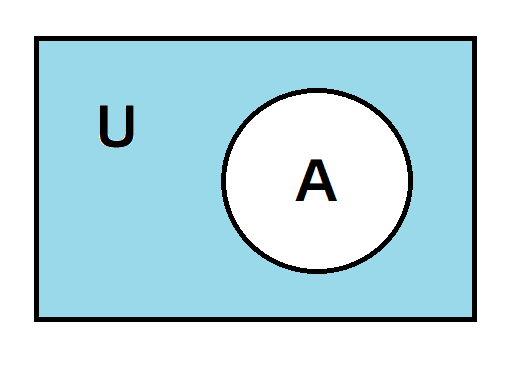
\includegraphics[width=0.2\textwidth]{image/Venn3.png}
  \caption{Venn图示例}
  \label{img:Venn3}
\end{figure}

\begin{example}
  设$U=\mathbb{R}$,则无理数集可以表示为$\overline{Q}$.
\end{example}

\begin{example}
  设$U=\mathbb{N}$,则$\overline{\mathbb{Z}^+}={0}$,这里的$\mathbb{Z}^+$表示正整数集。
\end{example}

下面是一个有趣的小例子。

\begin{example}
  设$A$为集合,则$\overline{\overline{A}}=A$.
\end{example}

还有一些其他的例子。

\begin{example}
  设$U=\{1,2,3,4,5,6\}$,$A=\{2,3,4\}$,则$\complement_{U}A=\{1,5,6\}.$
\end{example}

\begin{example}
  设$U=\mathbb{R},A=\{x\mid -1<x<6\}$,则$\complement_{U}A=\{x\mid x\leq -1\text{或}x\geq 6\}.$
\end{example}

\subsection{交集与并集}
下面来看看集合的运算。
有时候,我们需要研究两个集合的公共部分。比如说,不等式中每个不等式解集的公共部分就是整个不等式组的解集。
\begin{definition}[交集]
  设$A$,$B$为两个集合,由$A$和$B$中的公共元素所组成的集合称为$A$和$B$的
  \underline{交集},记作$A\cap B$,即$$A\cap B=\{x\in A\text{ 且 }x\in B\}.$$
\end{definition}
  交集可以理解为两个集合相交的部分。
  用Venn图表示如图\ref{img:Venn2}。
  \begin{figure}[h]
    \centering
    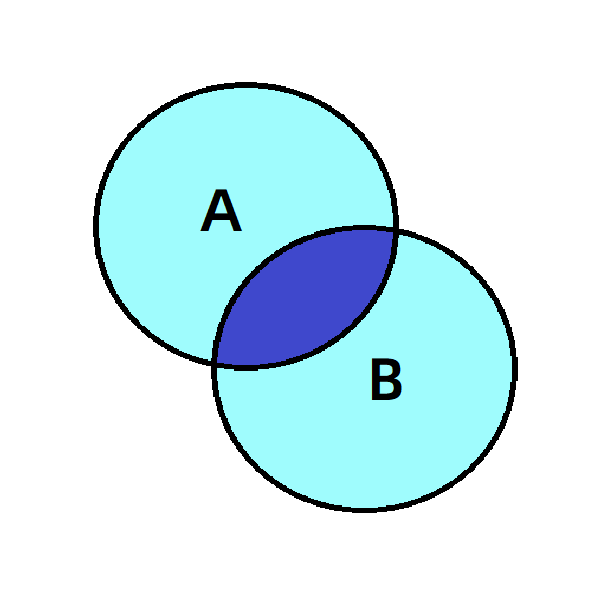
\includegraphics[width=0.2\textwidth]{image/Venn2.png}
    \caption{Venn图示例}
    \label{img:Venn2}
  \end{figure}
  图中深蓝色部分即为$A\cap B$。

\begin{definition}{并集}
  设$A$,$B$为两个集合,由$A$和$B$中所有元素组成的集合称为$A$和$B$的\underline{并集},记作$A\cup B$,即
  $$A\cup B=\{x\in A\text{或}x\in B\}$$
\end{definition}
  并集可以理解为两个集合合并且去掉重复元素后的部分。
  如图\ref{img:Venn2}所示,上色部分即为$A\cup B$。 

由这两个定义我们立刻可以得到这些常见的性质(更多的性质稍后介绍):

设$A$为集合,$U$为全集,则
\begin{property}
  零律:$A\cap\varnothing =\varnothing,A\cup\varnothing=A$;
\end{property}
\begin{property}
  同一律:$A\cap U=A;A\cup U=U$(这里$U$为全集).
\end{property}

\begin{exercise}\label{exer:10}
  用Venn图表示这两个定律。
\end{exercise}


这两个定律还是比较好理解的。所以我们直接快进到两个例子。

\begin{example}
  已知$A=\{1,2,3,4,5\},B=\{2,4,6\}$,则$A\cap B=\{2,4\}$,$A\cup B=\{1,2,3,4,5,6\}$.
\end{example}

\begin{example}
  若$A=\{\text{等腰三角形}\},B=\{\text{直角三角形}\}$,则$A\cap B=\{\text{等腰直角三角形}\}.$
\end{example}

\begin{example}
  已知集合$A=\{x|x^{2}+4x=0\},B=\{x\|x^{2}+2(a+1)x+a^{2}-1=0\}.$

  (1)若$A\cap B=B$,求实数$a$的取值范围;(2)若$A\cup B=B$,求实数$a$的取值范围。
\end{example}
\begin{remark}
  这道题目的关键就是如何理解两个小题各自给出的条件:

  $A\cap B=B$说明$A$最起码也包含$B$中的所有元素,即$B\subseteq A$,同样地,$A\cup B=B$即$A\subseteq B$.

  还有,不要忘了\textcolor{red}{讨论空集},这是集合当中的火坑(每年都有一大批人被坑)。
\end{remark}
\begin{solution}
  $A=\{x\mid x^{2}+4x=0\}=\{-4,0\}.$
  (1)$\because A\cap B=B,$\enspace$\therefore B\subseteq A.$
  
  若$0\in B$,则$a^2-1=0,a=\pm 1.$当$a=1$时,$B=A$;当$a=-1$时,$B=\{0\}$,均满足条件。

  若$-4\in B$,则$a^2-8a+7=0,a=7\text{ 或 }1.$当$a=7$时,$B=\{-12,-4\}\nsubseteq A$,不满足条件。

  若$B=\varnothing$,则$\Delta=4(a+1)^{2}-4(a^{2}-1)<0$,解得$a<-1$.

  综上,实数$a$的取值范围为$(-\infty,-1]\cup\{1\}.$

  (2)$\because A\cup B=B,$\enspace$A\subseteq B.$

  $\because A=\{-4,0\},$\enspace$\therefore B$中至少有两个元素$-4,0.$

  $\because B$中的元素为一元二次方程的实根,

  $\therefore B$中至多有2个元素,

  $\therefore A=B.$

  由(1)可知此时$a=1$.
\end{solution}
\begin{remark}
  请注意一下(1)中取值范围的写法,每一段用并集符号连接,如果一段只有一个值,需要用花括号括起来。
\end{remark}

\hspace*{\fill}

集合的交与并运算具有一些性质,前三个与四则运算的性质是相似的,但是有一些不同。

设$A,B,C$均为集合,则
\begin{property}
  交换律:$A\cup B=B\cup A,A\cap B=B\cap A$;
\end{property}
\begin{property}
  结合律:$A\cup(B\cup C)=(A\cup B)\cup C,A\cap(B\cap C)=(A\cap B)\cap C$;
\end{property}
\begin{property}
  分配律:$A\cap(B\cup C)=(A\cap B)\cup(A\cap C),A\cup(B\cap C)=(A\cup B)\cap(A\cup C)$;
\end{property}

  结合律的集合运算符号是相同的,分配律的集合运算符号是不同的,请注意区别。

\begin{property}
  吸收律:$A\cup(A\cap B)=A,A\cap(A\cup B)=A.$
\end{property}

\begin{exercise}
  用Venn图表示这些定律。
\end{exercise}

\hspace*{\fill}

我们在这里证明其中三个。

\begin{example}
  证明上面集合运算的结合律。
\end{example}
\begin{proof}
  $(A\cap B)\cap C=\{x|x\in A\cap B\text{ 且 }x\in C\}=\{x|x\in A\text{ 且 }x\in B\text{ 且 }x\in C\}=\{x|x\in A\text{ 且 }x\in B\cap C\}\\=A\cap(B\cap C).\\(A\cap B)\cap C=\{x|x\in A\cup B\text{ 或 }x\in C\}=\{x|x\in A\text{ 或 }x\in B\text{ 或 }x\in C\}=\{x|x\in A\text{ 或 }x\in B\cup C\}\\=A\cup(B\cup C).\hfill\square$
\end{proof}

\begin{remark}
  本书中,证明结尾的方框表示证明结束。
\end{remark}

\hspace*{\fill}

\begin{example}
  证明上面集合运算的分配律。
\end{example}

  和例\ref{exp:2}类似,我们用定义来证。但是这里只证明前一个,另外一个留作练习。

\begin{proof}
  首先证明$A\cap(B\cup C)\subseteq(A\cap B)\cup(A\cap C)$.

  \textcolor{cyan}{任取}\enspace$x\in A\cap(B\cup C)$,那么$x\in A\text{ 且 }x\in B\cup C$.

  若$x\in B$,由于$x\in A$,那么$x\in A\cap B$;

  若$x\in C$,由于$x\in A$,那么$x\in A\cap C$.

  所以$A\cap(B\cup C)\subseteq(A\cap B)\cup(A\cap C)$.

  \hspace*{\fill}

  再证明$(A\cap B)\cup(A\cap C)\subseteq A\cap(B\cup C)$.

  \textcolor{cyan}{任取}\enspace$x\in (A\cap B)\cup(A\cap C)$,那么$x\in A\cap B\text{ 或 }x\in A\cap C$.

  若$x\in A\cap B$,则$x\in B\cup C\text{且}x\in A$,所以$x\in a\cap(B\cup C)$;

  若$x\in A\cap C$,则$x\in B\cup C\text{且}x\in A$,所以$x\in a\cap(B\cup C)$.

  所以$(A\cap B)\cup(A\cap C)\subseteq A\cap(B\cup C)$.

  综上,$A\cap(B\cup C)=(A\cap B)\cup(A\cap C).\hfill\square$
\end{proof}
\begin{remark}
  请特别注意,我们需要“任取”,这样才比较严谨。
\end{remark}

\hspace*{\fill}

\begin{example}
  证明上面集合运算的吸收律。
\end{example}
关于这个定律的证明,我们使用的是引入其它集合(全集和空集)。

\begin{proof}
  $A\cup (A\cap B)=(A\cap U)\cup(A\cap B)=A\cap(B\cup U)=A\cap U=A.$

  (第二步逆用了分配律,最后两步用到了同一律。)

  $A\cap(A\cup B)=(A\cup\varnothing)\cap(A\cup B)=A\cup(B\cap\varnothing)=A.$

  (第二步逆用了分配律,最后一步用到了零律。)
\end{proof}

\subsection{习题}

\begin{exercise}\label{exer:11}
  集合$\{0\}$与$\varnothing$是否相等?它们满足什么关系?
\end{exercise}

\begin{exercise}\label{exer:12}
  证明:$\text{如果}A\subseteq B,B\subseteq S,\text{那么}A\subseteq S$.
\end{exercise}

\begin{exercise}\label{exer:20}
  $\text{设}U=\{\text{小于7的非负整数}\}\text{,}A=\{6\text{的正约数}\}\text{,}B=\{\text{不大于6的素数}\}\text{,}\text{求}\overline{A},\overline{A}\cap B, A\cup\overline{B}.$
\end{exercise}

\begin{exercise}\label{exer:19}
  $\text{设}U=\{x\mid x{\in}N,\text{且}x{\leqslant}10\},A=\{1,2,4,5,9\},B{=}\{4,6,7,8,10\},C=\{3,5,7\},\text{求:}\\A\cap B,A\cup B,\bar{A}\cap\bar{B},\bar{A}\cup\bar{B},(A\cap B)\cap C,(A\cup B)\cup C.$
\end{exercise}

\begin{exercise}\label{exer:14}
  $\text{已知}A=[-1,2],B=\left(-\infty,-\dfrac{p}{4}\right),\text{且}B\subsetneqq{\complement}_{\mathbb{R}}A\text{,求实数}p\text{的取值范围}.$
\end{exercise}

\begin{exercise}\label{exer:15}
  (1)证明:$\overline{A\cap B}=\overline{A}\cup\overline{B}$;
  (2)证明:$\overline{A\cup B}=\overline{A}\cap\overline{B}.$

  这是集合的De Morgan(德摩根)定律,这个定律可以推广到n个集合,这里不做推广,毕竟n个集合的并集定义还没给出。
\end{exercise}

\begin{exercise}\label{exer:16}
  我们记集合$A$的元素个数为$\mid A\mid$.

  (1)用Venn图说明:$|A\cup B|=|A|+|B|-|A\cap B|$.

  (2)用Venn图说明:$|A\cup B\cup C|=|A|+|B|+|C|-|A\cap B|-|B\cap C|-|C\cap A|+|A\cap B\cap C|$.

  (3)在$1,2,\cdots,100$中能被2,3或5整除的数共有多少个?

  这其实是集合的容斥原理,有兴趣的读者可查阅相关资料。
\end{exercise}

\begin{exercise}\label{exer:17}
  设$x,y,z$都是非零实数,试用列举法将$\dfrac x{|x|}+\dfrac y{|y|}+{\dfrac{z}{\mid z\mid}}+{\dfrac{xy}{\mid xy\mid}}+{\dfrac{xyz}{\mid xyz\mid}}$的所有可能值构成的集合表示出来.
\end{exercise}

\begin{exercise}\label{exer:18}
  设 A 是两个整数平方和的集合,即$A=\{x\mid x=m^2+n^2,\:m,\:n\in\mathbb{Z}\}.$

(1)证明:若 $s,t{\in}A$,则 $st{\in}A$;

(2)证明:若 s, $t\in A,t\neq0$,则$\dfrac st=p^2+q^2$,其中 $p,q$ 是有理数.
\end{exercise}

\section{命题、充分条件与必要条件}
本节只学习一些简易的逻辑,详细的逻辑学我们当然不可能在这里学到(好吧集合也是),如果你对逻辑学感兴趣,你可以阅读其他科普书或专业教材。

\subsection{命题的概念}

\begin{definition}{命题}
  \underline{命题},是可供真假判断的陈述语句。如果命题为真,我们称之为\underline{真命题};如果命题为假,我们称之为\underline{假命题}。
\end{definition}

\begin{remark}
  一个命题,要么是真命题,要么是假命题,不可能既真又假,也不可能不真不假。有的命题我们目前无法判断真假,如“不存在地外生命”,但它们确实是有真假的。
\end{remark}

命题也可以用符号和式子表示。比如说,命题”1小于2”可以表示为“$1<2$.

我们还可以用小写字母表示命题,比如说:$$p:1>2,$$

这显然是一个假命题。

习惯上,我们用$p,q,r,s,\cdots$表示命题.

\hspace*{\fill}

把一个命题的条件和结论互换就可以得到它的\underline{逆命题}。一个非常经典的例子是:“同位角相等,两直线平行”的逆命题是“两直线平行,同位角相等”.我们把像这样的两个命题称为\underline{互逆命题}。

\begin{remark}
  一个真命题的逆命题并不一定是真命题。
\end{remark}

\begin{exercise}\label{exer:202405021028}
  试着举出一个真命题,它的逆命题不是真命题。
\end{exercise}


\subsection{命题的判断与证明}

如果要判断一个命题为假命题,可以举一个\underline{反例},即举一个满足命题的条件,但不满足命题结论的例子。如果要判断一个命题为真命题就需要\underline{证明}了。

证明可以直接证明或者间接证明。直接证明有多种方法,我们将在未来的学习中逐步了解。间接证明的一种典型方法是\underline{反证法}。

反证法的基本步骤是这样的:

第一步,假设结论不成立(条件当然是要留着的)。

第二步,根据命题条件进行推理,得出矛盾。

第三步,通过矛盾得出否定后的结论不成立,从而肯定原来的结论。

这样就证明完了。

\hspace*{\fill}

现在来看一个例子。

\begin{example}
  求证:$\sqrt{2}$是无理数.
\end{example}
这是一个非常经典的命题。下面我们使用反证法来证明它。
\begin{proof}
  假设$\sqrt{2}$是有理数,那么$\sqrt{2}=\dfrac{p}{q}$(其中$p,q$互质,也就是说这是一个不可约分数,这是有理数的定义).

  两边平方,得$2=\dfrac{p^2}{q^2}$,即$2q^2=p^2$.

  因为$2q^2$为偶数,所以$p^2$为偶数,所以$p$为偶数.

  不妨设$p=2m$,则$2q^2=4m^2$,即$q^2=2m^2$,同上可知$q$也为偶数.

  这与$p,q$互质矛盾.

  因此$\sqrt{2}$是无理数.

\end{proof}

\subsection{推出关系、充分条件与必要条件}

\begin{remark}
  下面的内容极容易弄混,所以请务必仔细阅读。
\end{remark}

我们在初中就已经学过,数学中的命题经常写成“如果……,那么……”的形式,我们把它改成一般形式:
$$\text{如果}\alpha ,\text{那么}\beta.$$

其中的$\alpha$称为命题的\underline{条件},$\beta$称为命题\underline{结论}.

\begin{example}
  在命题“如果$x$是4的倍数,那么$x$是2的倍数”中,条件是“$x$是4的倍数”,结论是“$x$是2的倍数”。
\end{example}

\begin{exercise}
  在命题“三角形的内角和等于$180^{\circ}$”中,条件和结论分别是什么?
\end{exercise}

\hspace*{\fill}

接下来我们所要讨论的是不同命题之间的关系。

\begin{definition}{推出关系、等价命题}\label{def:tuichu}
  如果$\alpha$通过推理可以得出$\beta$,也就是“若$\alpha$,则$\beta$为真命题“,那么我们可以说“由$\alpha$可以推出$\beta$”,写成$\alpha\Rightarrow\beta$,读作“$\alpha$推出$\beta$”,其中的$\Rightarrow$叫做\underline{推出符号}。否则,我们说“由$\alpha$推不出$\beta$”,记作$\alpha\nRightarrow\beta$,读作“$\alpha$推不出$\beta$”。

  如果由$\alpha$可以推出$\beta$,由$\beta$也可以推出$\alpha$,那么我们称$\alpha$和$\beta$为\underline{等价命题},记作$\alpha\Leftrightarrow\beta$.
\end{definition}

\begin{example}\label{exp:202406231441}
  幼儿园的小朋友都知道,$4>2$,所以,$x>4\Rightarrow x>2$.
\end{example}

\begin{problem}\label{202406262000}
  参考例\ref{exp:202406231441},思考怎样从集合的观点理解推出关系。
\end{problem}

此外,推出关系具有\underline{传递性},也就是说,如果$\alpha\Rightarrow\beta,\beta\Rightarrow\gamma,$那么$\alpha\Rightarrow\gamma$.

\hspace*{\fill}

现在我们接着定义\ref{def:tuichu},我们将要给出两个重要的概念。

\begin{definition}{充分条件与必要条件}
  如果$\alpha\Rightarrow\beta$,称$\alpha$是$\beta$的\underline{充分条件},$\beta$是$\alpha$的\underline{必要条件}。

  同理,如果$\alpha\nRightarrow\beta$,称$\alpha$不是$\beta$的充分条件,$\beta$不是$\alpha$的必要条件。
\end{definition}

\begin{quotation}
  【掩体纪元67年,“星环号”】

  “打击警报出现了吗?”程心问,曹彬点点头。

  ……

  “为什么还不进掩体?!”AA指着舷窗外的太空城组合体问。

  “没有\underline{\textbf{必要}}了,掩体没用。”曹彬垂下眼睛说。

  “光粒现在距太阳有多近了?”程心问。

  “没有光粒。”

  “那你们发现了什么?”

  曹彬凄惨地笑了起来,“一张小纸条。”

——刘慈欣《三体3:死神永生》
\end{quotation}

现在就有一个问题了,我们前面所学的四个概念(现在列在下面):
\begin{itemize}
  \item “如果$\alpha$,那么$\beta$”是真命题;
  \item $\alpha\Rightarrow\beta$;
  \item $\alpha$是$\beta$的充分条件;
  \item $\beta$是$\alpha$的必要条件,
\end{itemize}

这四个表达有什么关系呢?

回答是,它们没有本质上的区别,讲的都是同一个逻辑关系。

数学这个东西,很多时候都是这样,你会看到许多说法不同,但本质一样的表达。

\hspace*{\fill}

先举两个例子:

\begin{example}\label{202406262001}
  因为$x=y\Rightarrow x^2=y^2$,所以"$x=y$"是"$s^2=y^2$"的充分条件,"$s^2=y^2$"是"$x=y$"的必要条件。
\end{example}

\begin{example}\label{202406262002}
  因为$x$是矩形$\nRightarrow x$是正方形,所以“$x$是矩形”不是“$x$是正方形”的充分条件,“$x$是正方形”不是“$x$是矩形”的必要条件。

  但是,反过来就不一样了。在这里,因为$x$是正方形$\Rightarrow x$是矩形,所以“$x$是正方形”是“$x$是矩形”的充分条件,“$x$是矩形”是“$x$是正方形”的必要条件。
\end{example}

来几道简单的练习。

\begin{exercise}\label{202406262010}
  判断下列各题中,$p$是否是$q$的充分条件,$q$是否是$p$的必要条件:

  (1)$p:x\in\mathbb{Z},q:x\in\mathbb{R}$;

  (2)$p:a=b,q:ac=bc$;

  (3)$p:$两个三角形全等,$q:$两个三角形面积相等.
\end{exercise}

\begin{exercise}\label{202406262101}
  判断下列“若p,则q”形式的命题当中,哪些命题中的p是q的充分条件,或者说q是p的必要条件?

  (1)若四边形的两组对角分别相等,则这个四边形是平行四边形;

  (2)若四边形为菱形,则这个四边形的对角线互相垂直;

  (3)若$x,y$为无理数,则$xy$为无理数;

  (4)若直线$l$与$\odot O$有且仅有一个交点,则$l$为$\odot O$的一条切线;

  (5)若$x,y$都能被5整除,则$x+y$也能被5整除;

  \begin{spacing}{2.0}
    (6)如果$\dfrac{a}{b}=\dfrac{c}{d}$,则$\dfrac{a+b}{b}=\dfrac{c+d}{d}$.
  \end{spacing}
\end{exercise}

\hspace*{\fill}

下面我们将要了解更复杂一点的内容。

我们知道,$x=y\Rightarrow x^2=y^2$,但是$x^2=y^2\nRightarrow x=y$,所以$x=y$是$x^2=y^2$的充分条件,但不是$x^2=y^2$的必要条件。

我们尝试把这两个说法合在一起:

$$x=y\text{是}x^2=y^2\text{的}\textbf{充分不必要条件。}$$

\begin{definition}
  如果$\alpha\Rightarrow\beta$,且$\beta\nRightarrow\alpha$,则称$\alpha$是$\beta$的\underline{充分不必要条件}。

  如果$\alpha\nRightarrow\beta$,且$\beta\Rightarrow\alpha$,则称$\alpha$是$\beta$的\underline{必要不充分条件}。

  如果$\alpha\nRightarrow\beta$,且$\beta\nRightarrow\alpha$,则称$\alpha$是$\beta$的\underline{既不充分也不必要条件}。

  如果$\alpha\Rightarrow\beta$,且$\beta\Rightarrow\alpha$,则称$\alpha$是$\beta$的\underline{充分必要条件},简称\underline{充要条件},记作$\alpha\Leftrightarrow\beta$,也可以读作“$\alpha$与$\beta$等价”或“$\alpha$当且仅当$\beta$”。
\end{definition}

\begin{remark}
  $\alpha$是$\beta$的充要条件时,$\beta$也是$\alpha$的充要条件。
\end{remark}

\hspace*{\fill}

\begin{example}
  在$\triangle ABC$中,$\angle B=\angle C$是$AC=AB$的充要条件。
\end{example}

\begin{example}
  “$A\subseteq B$且$B\subseteq A”$是$A=B$的充要条件。
\end{example}

\begin{example}
  $xy=0$是$x=0$的必要不充分条件。
\end{example}

\begin{example}
  “两个三角形全等”是“两个三角形的对应角相等”的充分不必要条件。
\end{example}

\begin{example}
  $x>y$是$x^2>y^2$的既不充分也不必要条件。
\end{example}

\begin{example}
  数学中的定义给出的是一个充要条件(如“两组对边分别平行的四边形是平行四边形”)。
\end{example}

\hspace*{\fill}

最后来看一个综合一些的例子。

\begin{example}\label{2022BST_Math_BX1_RJA_P18.20}
  已知集合$P=\left\{x|-2\leq x\leqslant10\right\}$,非空集合$S=\left\{x|1-m\leqslant x\leqslant1+m\right\}.$

  (1)若$x\in P$是$x\in S$的必要条件,求实数$m$的取值范围;

  (2)是否存在实数$m$,使$x\in P$是$x\in S$的充要条件?
\end{example}

\begin{solution}
  (1)$\because x\in P$是$x\in S$的必要条件,$\therefore S\subseteq P$,

  $\therefore\begin{cases}1-m\leqslant1+m\:,\\1-m\geqslant-2\:,\\1\:+m\leqslant10\:,\end{cases}$
  
  $\therefore 0\leqslant m\leqslant 3,$
  即实数$m$的取值范围是$\left\{m|0\leqslant m\leqslant3\right\}.$

  (2)若$x\in P$ 是$x\in S$ 的充要条件,则$P=S$,

  $\therefore\begin{cases}1-m=-2,\\1+m=10,\end{cases}$
  
  方程组无解,即不存在实数 $m$,使 $x\in P$ 是$x\in S$ 的充要条件。
\end{solution}

\subsection{充分、必要条件的证明}

这部分其实就一句话:根据条件和要求,把是否充分和是否必要分别证出来就可以了。

\begin{example}\label{HS2FZ_lkb1_P26.1}
  求证:“$b^2-4ac=0$”是“关于$x$的实系数一元二次方程$ax^2+bx+c=0$有两个相等的实数根”的充要条件。
\end{example}

\begin{proof}
  先证充分性,

  原方程可化为$\left(x+\dfrac{b}{2a}\right)^{2}=\dfrac{b^{2}-4ac}{4a^{2}}$,

  当$b^2-4ac=0$时,上式右边等于0,则原方程有两个相等的实数根$x_1=x_2=-\dfrac{b}{2a}$.

  再证必要性,
  
\begin{spacing}{1.8}
  若关于$x$的实系数一元二次方程$ax^2+bx+c=0$有两个相等的实数根,则由一元二次方程根与系数的关系可得$x_{1}+x_{2}=2x_{1}=-\dfrac{b}{a},x_{1}x_{2}=x_{1}^{2}=\dfrac{c}{a},$

  因此$\left(-\dfrac{b}{2a}\right)^{2}=\dfrac{c}{a}$,即$b^2-4ac=0$.
\end{spacing}

\end{proof}

\subsection{习题}

\begin{exercise}\label{2017RJB_bx1_P26}
  判断下列命题的真假:

  (1)存在两个无理数,它们的乘积是有理数;

  (2)没有一个无理数不是实数;

  (3)集合$A$是集合$A\cup B$的子集;

  (4)集合$A\cap B$是集合$A$的子集;

\begin{spacing}{2.0}
    (5)如果$\dfrac ab=\dfrac cd$,则$\dfrac{a+b}b=\dfrac{c+d}{d}$;

  (6)一元三次方程都有三个不同的实数根;
  
  (7)如果$\dfrac ab=\dfrac cd\neq 1$,则$\dfrac a{b-a}=\dfrac c{d-c}$.
\end{spacing}

\end{exercise}

\begin{exercise}\label{202407081520}
  证明:$\sqrt{3}$是无理数。
\end{exercise}

\begin{exercise}\label{BJ4Z_Algebra1_P28.2}
  用“充要”“充分不必要”“必要不充分”“既不充分也不必要”填空(本题中默认$a\in\mathbb{R},b\in\mathbb{R}$):

  (1)$a^2=b^2$是$a=b$的\underline{\hbox to 15mm{}}条件;

  (2)$a^3=b^3$是$a=b$的\underline{\hbox to 15mm{}}条件;

  (3)使$ab=0$的充分条件是\underline{\hbox to 15mm{}};

  (4)使$ab=0$的必要条件是\underline{\hbox to 15mm{}};

  (5)使$ab\neq 0$的充要条件是\underline{\hbox to 15mm{}};

  (6)“$a>2$”是“$a\geqslant2$”的\underline{\hbox to 15mm{}}条件;

  (7)“$a、b$不全是0”是“$a、b$全不是0”的\underline{\hbox to 15mm{}}条件;

  (8)“$\vert a-2\vert\neq2-a$”是“$a\geqslant2$”的\underline{\hbox to 15mm{}}条件。
\end{exercise}

\begin{exercise}\label{2017_XJ_bx1_P23.8}
  已知$p$是$r$的充分条件,$r$是$q$的必要条件,同时也是$s$的充分条件,$q$是$s$的必要条件,那么:
\end{exercise}

\begin{enumerate}
  \item $s$是$p$的什么条件?
  \item $p$是$q$的什么条件?
  \item 在$p,q,r,s$中,哪几对互为充要条件?
\end{enumerate}

\begin{exercise}\label{2017_RJB_bx1_P36.B5}
  已知$A=(-\infty,a]$,$B=(-\infty,3)$,且$x\in A$是$x\in B$的充分不必要条件,求$a$的取值范围。
\end{exercise}

\begin{exercise}\label{zhw2000_g1_P51.78}
  求证:关于$x$的方程$ax^2+bx+1=0$有一根为1的充要条件是$a+b+c=0$.
\end{exercise}

\section{量词、逻辑连接词与四种命题形式}

在前面我们已经学习了几个逻辑用语:命题、推出、充分条件和必要条件。

接下来则是几个新的逻辑用语。

\subsection{量词}

我们有时候会遇到一些含有变量的语句,由于变量的取值不确定,这些语句的真假性是无法判断的。比如说:

$$x>0;$$

$$x^2+y^2=1.$$

像这样含有变量的语句称为\underline{开语句}或者\underline{条件命题}。

但是,倘若我们给开语句的变量赋值以后,情况就不一样了。

比如说,“如果$x=5,x>0$”是一个真命题。

我们还可以在开语句前加上其他条件,比如说:

$$\text{对所有正整数}x,2x+3\text{是正整数。}$$

这也是一个命题,它的特别之处在于含有“所有”这个词。逻辑学当中,我们称它为\underline{全称量词},记作“$\forall$”。含有全称量词的命题称为\underline{全称量词命题}。

我们将上面的命题用符号表示:

$$\forall x\in\mathbb{N}^*,2x+3\in\mathbb{N}^*.$$

一般来说,全称量词命题即为形如“对集合$M$中的所有元素$x$,$p(x)$”的命题(这里的$p(x)$是一个有关$x$的陈述语句),可以简记为“$\forall x\in M,p(x)$”.

\hspace*{\fill}

我们还要提到一个量词:\underline{存在量词}。

全称量词的意思就是“存在”,记作“$\exists$”,含有存在量词的命题称为\underline{存在量词命题}。

例如,命题“存在$x>3$,使得$4x-7>0$”就是一个存在量词命题,用符号表示为:

$$\exists x>3,4x-7>0.$$

一般来说,存在量词命题即为形如“存在集合$M$中的元素$x$,$p(x)$”的命题,可以简记为“$\exists x\in M,p(x)$”.

现在,我们来考虑一个问题:如何判定全称量词命题和存在量词命题的真假?

对于全称量词命题,要判断其为真,需要验证集合$M$中的所有元素都满足$p(x)$,要判断其为假,只需要举出一个反例即可;

对于存在量词命题,要判断其为真,只需要举出一个满足$p(x)$的$x$即可,要判断其为假,需要验证集合$M$中的所有元素都不满足$p(x)$.

作为全称量词和存在量词的应用,我们现在给出若干集合的并集和交集的表示方法(这些集合的个数可以有限,也可以无限):

\begin{definition}{集合族}
  以集合为元素的集合称为\underline{集合族}或\underline{集合类}。
\end{definition}

\begin{definition}{若干个集合的并集}
  设$\{E_\alpha\mid\alpha\in I\}$(其中$\alpha$称为\underline{指标},$I$是由全体指标构成的\underline{指标集},指标集可以是有限集,也可以是无限集),则这些集合$E_\alpha$的并集定义为$$\bigcup_{\alpha\in I}E_\alpha=\{x\mid\exists\alpha\in I,x\in E_\alpha\}$$
\end{definition}

\begin{definition}{若干个集合的交集}
  设$\{E_\alpha\mid\alpha\in I\}$(其中$I$为指标集),则这些集合$E_\alpha$的交集定义为$$\bigcap_{\alpha\in I}E_\alpha=\{x\mid\forall\alpha\in I,x\in E_\alpha\}$$
\end{definition}

你在学习数学上的$n$维空间时一定会用到这两个概念。

\subsection{逻辑联结词}

我们在定义交集和并集的时候用到了“且”和“或”两个逻辑联结词,此时我们只能从日常语言角度理解它们。现在我们从逻辑学角度解释一下它们的用法。

\subsubsection{且}

生活中,人们经常用“且”表示“同时满足”,如公司招聘要求中写“18-55岁\textcolor{red}{且}具有大专学历”。(当然“且”这个字还有别的意思,比如表并列。)

逻辑学中,我们用“且”联结两个命题$p$和$q$,得到的新命题记作“$p\land q$,读作“$p$且$q$”.

我们规定,当$p$和$q$均为真时,$p\land q$为真;当$p$和$q$中至少有一个为假时,$p\land q$为假。这和日常语言中的“且”是一样的。

\subsubsection{或}

“或”和“或者”也是在生活中经常被使用的字词。

逻辑学上,我们用“或”联结两个命题$p$和$q$,得到的新命题记作“$p\lor q$,读作“$p$或$q$”。

我们规定,如果$p$和$q$中至少有一个为真,则$p\lor q$为真,如果$p$和$q$均为假,则$p\lor q$为假。这和日常语言中的“或”“或者”并不完全相同。

\hspace*{\fill}

\begin{example}
  将下列各组命题分别用“且”和“或”联结为新命题,并判断真假。
\end{example}

(1)$p$:正方形的对角线相等;$q$:正方形的对角线互相垂直。

(2)$p$:1是素数;$q$:2是素数。

\begin{solution}
  (1)$p\land q$:正方形的对角线相等且互相垂直;$p\lor q$:正方形的对角线相等或互相垂直。因为$p$和$q$都是真命题,所以$p\land q$是真命题,$p\lor q$也是真命题。

  (2)$p\land q$:1是素数且2是素数;$p\lor q$:1是素数或2是素数。因为$p$是假命题,$q$是真命题,所以$p\land q$是假命题,$p\lor q$是真命题。
\end{solution}

\subsubsection{非(否定)}

对一个命题$q$的\textcolor{blue}{结论}进行否定,得到的新命题记作“$\neg q$”,读作“非$q$”或者“$q$的否定”。我们规定,$p$和$\neg q$的真假\underline{相反}。

\begin{remark}
  请和后文的“否命题”进行区别。
\end{remark}

\begin{example}
  命题“我现在的年龄是16岁”的否定是“我现在的年龄不是16岁”。
\end{example}

\begin{example}
  命题“$x^2+2x+2>0$”的否定是$x^2+2x+1\leq 0$”.
\end{example}

\subsection{如何正确地写出命题的否定}

如果一个命题中含有全称量词或者存在量词,在写它的否定时需要做出一些改变。

先来看两个例子:

命题“所有的数都是有理数”的否定是“不是所有的数都是有理数”,换一个说法,就是“存在不是有理数的数”。这里的\textcolor{red}{全称量词}在否定后变为了\textcolor{blue}{存在量词}。

命题“存在无实数解的一元二次方程”的否定是“所有一元二次方程都有实数解”。这里的\textcolor{blue}{存在量词}在否定后变为了\textcolor{red}{全称量词}。

把上面的内容一般化。“$\exists x\in M, p(x)$”的否定是“$\forall x{\in}M,\neg p(x)$”,“$\forall x\in M, q(x)$”的否定是“$\exists x{\in}M, \neg q(x)$”.

\begin{example}
  命题“$\forall x>1,x+2>3$”的否定是“$\exists x>1,x+2\leqslant 3$”.
\end{example}

\begin{example}
  命题“$\exists x\in\mathbb{R},x^2-1\geqslant 0$”的否定是“$\forall x\in\mathbb{R},x^2-1<0$”.
\end{example}

命题中含有“且”“或”时,书写它的否定也需要注意。

$p\land q$的否定形式为$\lnot p\lor \lnot q$,$p\lor q$的否定形式为$\lnot p\land \lnot q$.

就是说,书写含“且”“或”的命题的否定时,记得把“且”和“或”换一下。

\begin{example}
  命题“若$x=1$或$x=2$,则$x(x-1)=0$或$x(x-2)=0$”的否命题是“若$x\neq 1$且$x\neq 2$,则$x(x-1)\neq 0$且$x(x-2)\neq 0$”.
\end{example}

\subsection{四种命题形式}

我们先给出一个命题:

\begin{equation}\label{YuanMingTi}
  \text{如果}p\text{,则}q.
\end{equation}

我们将这个命题作为\underline{原命题},也就是原本的命题。

现在我们对它做一些变换:

将条件和结论互换,就得到原命题的\underline{逆命题}(两者为\underline{互逆命题}):

\begin{equation}\label{NiMingTi}
  \text{如果}q\text{,则}p.
\end{equation}

分别否定条件和结论,就得到原命题的\underline{否命题}(两者为\underline{互否命题}):

\begin{equation}\label{FouMingTi}
  \text{如果}\neg p\text{,则}\neg q.
\end{equation}

将条件和结论互换并分别否定,就得到原命题的\underline{逆否命题}(两者\underline{互为逆否命题}):

\begin{equation}\label{NiFouMingTi}
  \text{如果}\neg q\text{,则}\neg p.
\end{equation}

这就是命题的四种形式。

命题的形式是相对的。

如果我们将命题\ref{NiMingTi}看作原命题,那么命题\ref{YuanMingTi}就是它的逆命题。也就是说,命题\ref{YuanMingTi}和\ref{NiMingTi}\textbf{互为}逆命题。其余同理。

我们用一张图来表示以上的关系:

\begin{figure}[h]
  \centering
  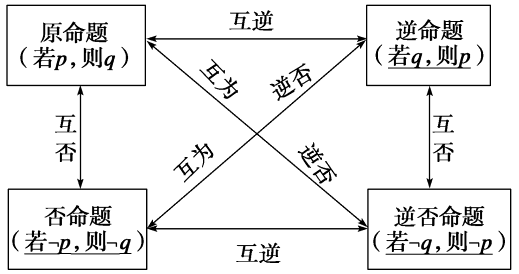
\includegraphics[width=0.4\textwidth]{image/proposition.png}
  \caption{命题图示(来源网络)}
  \label{img:proposition}
\end{figure}

此外,我们给出四种命题的真假性关系。

\begin{itemize}
  \item 两个命题互为逆否命题,它们的真假性相同;
  \item 两个命题为互逆命题或互否命题,它们的真假性无关。
\end{itemize}

\begin{problem}
  举出这样的例子。
\end{problem}

\subsection{取逆否命题证明}

由上一小节最后的真假关系,我们不难想到,倘若直接证明一个命题有难度,我们可以考虑证明它的逆否命题。这是一种“正难则反”的操作。

直接举一个例子。

\begin{example}
  判断命题“如果$x+y\neq 3$,那么$x\neq 1$或$y\neq 2$的真假。
\end{example}

\begin{solution}
  该命题的逆否命题为:如果$x=1$且$y=3$,那么$x+y=3$.显然为真命题。所以原命题也为真命题。
\end{solution}

\subsection{习题}

\begin{exercise}
  用数学符号写出下列命题并判断真假:
\end{exercise}

\begin{enumerate}
  \item 所有实数的平方都是正数;
  \item 存在两个无理数,它们的乘积是有理数;
  \item 三个连续整数的乘积是6的倍数;
  \item 大于3的自然数是不等式$x^2>10$的解。
\end{enumerate}

\begin{exercise}
  判断下列命题的真假,并写出这些命题的否定(请注意这里有些命题\textcolor{blue}{省略了全称量词}):
\end{exercise}

\begin{enumerate}
  \item 至少有一个整数$n$,$n^2+1$是4的倍数;
  \item 每个二次函数的图像都是轴对称图形;
  \item 存在一个四边形,它的四个顶点不共圆;
  \item 若$x>1$,则$2x+1>5$;
  \item 若四边形为等腰梯形,则这个四边形的对角线相等;
  \begin{spacing}{1.7}
     \item $\forall x{\in}\mathbb{R}$,$\dfrac1{x^2+1}{<}1$;
  \end{spacing}
   \item $\forall a,b{\in}\mathbb{R}$,$a^3+b^3=(a+b)(a^2-ab+b^2)$.
\end{enumerate}

\begin{exercise}
  判断下列命题的真假:
\end{exercise}

\begin{enumerate}
  \item $\forall x\in(-1, 2), x\in[-1, 2)$;
  \item $\forall x\in\mathbb{Q}, |x|+x\geqslant0$;
  \item $\exists x,y\in\mathbb{Z},3x-2y=10$;
  \item 集合$A$是集合$A\cup B$的子集;
  \item 集合$A\cap B$是集合$A$的子集;
  \item 存在有序整数组$(x,y)$满足$xy=x+y$.
\end{enumerate}

\begin{exercise}
  用联结词“且”和“或”分别联结下面各组命题组成新命题,并判断它们的真假:
\end{exercise}

\begin{enumerate}
  \item $p$:$17<20$;$q$:$17=20$.
  \item $p$:平行四边形对角线互相平分;$q$:平行四边形的对角线相等。
  \item $p$:4是素数;$q$:4不是奇数;
  \item $p$:能被5整除的整数的个位数一定为5;$q$:能被5整除的整数的个位数一定为0。
\end{enumerate}

\begin{exercise}
  写出下列命题的非:
\end{exercise}

\begin{enumerate}
  \item $\forall x\in\mathbb{R},3x=2x+x$;
  \item $\exists x\in\mathbb{N},x^2=x+2$;
  \item 至少有一个锐角$\alpha$,使$\sin\alpha=0$;
  \item $a,b$都是有理数。
\end{enumerate}

\begin{exercise}
  写出下列命题的逆命题、否命题和逆否命题并判断真假:
\end{exercise}

\begin{enumerate}
  \item 线段的垂直平分线上的点到这条线段两个端点的距离相等;
  \item 矩形的对角线相等;
  \item 如果$x=y=0$,那么$(x-y)(x+y)=0$;
  \item 对顶角相等。
\end{enumerate}

\begin{exercise}\label{2003RJA_xx2-1_P7.exp4}
  证明:若$x^2+y^2=0$,则$x=y=0$.
\end{exercise}

\section{全章综合回顾}

\subsection{补充材料}

\subsubsection{de Morgan定律}

\subsubsection{Russell悖论}

\subsection{习题}

\chapter{函数}

\epigraph{不借助函数却想去做微积分,这无疑会是你所能做的最无意义的事情之一.如果微积分也有其营养成分表,那么函数肯定会排在最前面,而且是占一定优势.}{《普林斯顿微积分读本》}

在开始讲函数之前,我们先来看看函数的历史(更具体的可参见《古今数学思想(第一册)》和《古今数学思想(第四册)》(Morris Kiline著),此处对此作一些概括)。

首先是Galileo(伽利略,1564-1642)。Galileo在其著作《两门新科学》中,用文字和比例的语言表达函数关系。随着代数符号化的发展,不久后他就用$s=kt^2$来表示落体距离(放在现在就类似于自由落体运动的下落距离$h=\dfrac{1}{2}gt^2$)。

十七世纪,James Gregory(格雷戈里,1638-1675)在其论文《论圆和双曲线的求积》中定义函数为这样一个量:它是从一些其他的量经过一系列代数运算而得到的,或者经过任何其他可以想象到的运算而得到的。

此外,Newton(牛顿,1643-1727)用“流量”一词表示变量间的关系,Leibniz(莱布尼茨,1646-1716)用“函数”表示任何一个随着曲线上的点的变动而变动的量(如切线和纵坐标)。后来的Lagrange则用“函数”一词表示几乎是任意类型的对一个或多个变量的依赖关系。

1734年,Euler(欧拉,1707-1783)引进了记号$f(x)$,这也是我们现在所使用的记号。

1887年,Dedekind(戴德金,1831-1916)给出了“映射”的概念。现阶段,我们使用映射来定义函数。

\section{映射与函数}

\subsection{映射/函数的定义}

开头先说明一下,\textbf{映射也称为函数}。

我们先给出映射的定义以及几个注释,再给例子。

\begin{definition}{映射/函数}
  设$A,B$是两个非空集合,若存在一个对应法则$f$,使得对$A$中的每个元素$x$,在$B$中都有\textcolor{orange}{唯一确定}的元素$y$按法则$f$与之对应(可以多对一,也可以一对一,但不能一对多),则称$f$为从$A$到$B$的\underline{映射}或从$A$到$B$的\underline{函数},记作$$f:A\rightarrow B,y=f(x)\text{或}f:A\rightarrow B,x\mapsto f(x)$$其中$y$称为元素$x$(在映射$f$下)的\underline{像},或者称为$x$对应的\underline{函数值},记作$f(x)$;元素$x$称为元素$y$(在映射$f$下)的\textcolor{orange}{一个}\underline{原像};集合$A$称为映射$f$的\underline{定义域},$A$中所有元素的像组成的集合称为映射$f$的\underline{值域}。

  若我们知道$f(x)$的表达式(如\ref{MapExample2}),则使得$f(x)$有意义的所有$x$组成的集合称为\underline{自然定义域}。
\end{definition}

\begin{remark}
  考虑到一元函数(按初中理解方式,就是只有一个变量的函数,我们接下来就要讨论这个)和多元函数(有多个变量的函数,本读本可能不讲)的统一,我们采用了这种广义的定义方式。
\end{remark}

\begin{remark}
  值域也可以这样表示:$$\left\{f(x)\mid x\in A\right\}.$$
\end{remark}

\begin{remark}
  集合中的元素不一定是一个数!!!
\end{remark}

下面我们给出一元函数的定义。

\begin{definition}{一元函数}
  若集合$D\subseteq \mathbb{R}$,则我们称函数$f:D\rightarrow\mathbb{R}$为\underline{一元函数}。
\end{definition}

\textcolor{blue}{此后,若无特殊说明,本读本中的函数均指的是一元函数。}

举几个例子。

\begin{example}
  我们设$A=\left\{1,-1,2,-2,3,-3\right\}$,$B=\left\{1,4,9\right\}$,对应法则为“平方”,则我们可以画出下图表示从$A$到$B$的映射:
\end{example}

\begin{figure}[h]
  \centering
  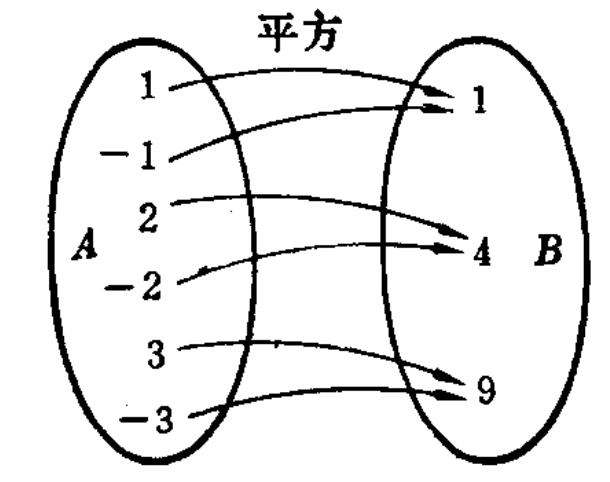
\includegraphics[width=0.2\textwidth]{image/map2.1.1.png}
  \caption{一个对应法则为“平方”的映射(图源:《高级中学课本(试用) 代数 第一册(甲种本)》)}
  \label{img:map1}
\end{figure}

\begin{example}\label{MapExample2}
  让每一个$x\in\mathbb{R}$对应$2x$,就可以给出一个从$\mathbb{R}$到$\mathbb{R}$的映射$$f:\mathbb{R}\rightarrow\mathbb{R},f(x)=2x.$$我们将其写成这样的形式(下文同):$$f(x)=2x(x\in\mathbb{R}).$$这里的$(x\in\mathbb{R})$由于是自然定义域,通常省去不写,直接写$f(x)=2x$,\textcolor{blue}{读作}“$fx$等于$2x$”。

  举个代入$x$值的例子。当$x=2$时,$f(2)=2\times 2=4$.
\end{example}

\begin{spacing}{2.0}
  \begin{example}
    函数$f(x)=\dfrac{2}{x}$的自然定义域是$(-\infty,0)\cup(0,+\infty)$,此时的值域是$(-\infty,0)\cup(0,+\infty)$.
  \end{example}
  
  \begin{example}
    函数$f(x)=\dfrac{1}{\sqrt{x-1}}$的自然定义域是$(1,+\infty)$,值域是$(0,+\infty)$.
  \end{example}
  
  下面是更具体一些的例子。
  
  \begin{example}
    求下列函数的自然定义域:
  \end{example}
  
  \begin{enumerate}
    \item $f(x)=\dfrac{\sqrt{x}+2}{\sqrt{x}-3}$;
    \item $f(x)=\dfrac{3x}{\left| x \right|-x}$.
  \end{enumerate}
\end{spacing}

\begin{solution}
  \begin{enumerate}
    \item 函数$f(x)$有意义当且仅当
     $\begin{cases}
        x>0
        \\\sqrt{x}-3\neq 0
      \end{cases}$
    ,解得$0<x<9$或$x>9$,所以$f(x)$的定义域为$(0,9)\cup (9,+\infty)$.

    \item 函数$f(x)$有意义当且仅当$\left| x \right|\neq x$,即$x<0$,所以$f(x)$的定义域为$(-\infty,0).$
  \end{enumerate}
\end{solution}

\begin{spacing}{2.0}
  \begin{example}
    求下列函数的值域:
  \end{example}
  
  \begin{enumerate}
    \item $f(x)=\dfrac{\sqrt{x}+2}{\sqrt{x}-3}$;
    \item $y=2x-\sqrt{x-1}$;
  \end{enumerate}
\end{spacing}

给出解法之前先说明一下,函数的记号不一定要用$f(x)$,也可以用其他字符表示不同的对应关系,比如说$g(x),\phi (x)$,甚至是$Loss(x)$,如果定义域中的元素记号也用其它字符表示,比如$y$,那么就可以写成类似$f(y),g(y)$的形式。不同的记号用来表示不同的函数,可以有效避免混淆。

\begin{solution}
  \begin{enumerate}
    \item $f(x)=\dfrac{\sqrt{x}+2}{\sqrt{x}-3}=1+\dfrac{5}{\sqrt{x}-3}$,
    
    令$y=\sqrt{x}-3$,则$y$的取值范围为$[-3,0)\cup (0,\infty)$,再令$g(y)=\dfrac{5}{y}$,由初中反比例函数的知识可得$g(y)$的值域为$(-\infty,-\dfrac{5}{3}]\cup (0,+\infty)$.

    因为$f(x)=1+g(y)$,所以$f(x)$的值域为$(-\infty,-\dfrac{2}{3}]\cup (1,+\infty)$.

    \item 令$t=\sqrt{x-1}$(换元),则$t\geqslant 0,x=t^2+1,y=2t^2-t+2=2(t-\dfrac{1}{4})^2+\dfrac{15}{8}\geqslant\dfrac{15}{8}$,\textcolor{blue}{当且仅当$t=\dfrac{1}{4}$时等号成立}。所以函数的值域为$[\dfrac{15}{8},+\infty).$
  \end{enumerate}
\end{solution}

\begin{spacing}{2.0}
  \textbf{定义域、对应法则、值域}是函数的三要素。但是,函数不一定能用公式或图像表示。比如说下面的两个例子。
\end{spacing}

\begin{example}
  Euler(欧拉)函数$\phi (n)$表示小于等于$n$且和$n$互质的数的个数。我们并不能写出这个函数的表达式,但是这样一个对应关系确实满足函数的定义。
\end{example}

下面的函数我们采用分段表示(写成\underline{分段函数}的形式),写法是先写表达式,然后写一个逗号,在逗号后加上取值范围。

\begin{example}
  Dirichlet(狄利克雷)函数定义为
  $$f(x)=
  \begin{cases}
    1,x\in\mathbb{Q}
    \\0,x\in\complement_{\mathbb{R}}\mathbb{Q}
  \end{cases},$$
  这个函数我们能写出表达式,但是画不出图像(图像的问题我们后面讨论)。
\end{example}

最后来看一个有趣的函数。

\begin{example}
  符号函数$sgn(x)$定义为
  $$sgn(x)=
  \begin{cases}
    1,x>0
    \\0,x=0
    \\-1,x<0
  \end{cases},$$
\end{example}

\subsection{单射、满射与一一映射}

\begin{definition}{映射的相等}
  设$f:A\rightarrow B$,且$g:A\rightarrow B$,若$\forall x\in A,f(x)=g(x)$,则称映射$f$和$g$是\underline{相等}的。记作$f=g$.
\end{definition}

通俗地解释就是三要素相同。

\begin{example}
  函数$y=x$和$y=\sqrt{x^2}$相等,和$u=\sqrt[3]{x^3}$相等,但和$y=\dfrac{x^2}{x}$不相等,因为定义域和值域不同。
\end{example}

\begin{definition}{单射}
  设$f:A\rightarrow B$,若对任意$x,y\in A$,且$x\neq y$,有$f(x)\neq f(y)$,则称$f$为\underline{单射}。
\end{definition}

也就是说,不同的$x$所对应的函数值都不相等。如$f(x)=2x$,$g(x)=\dfrac{1}{x}$.

\begin{definition}{满射}
  设$f:A\rightarrow B$,若$f$的值域与$B$相等,则称$f$为从$A$到$B$的\underline{满射}。
\end{definition}

也就是说,$B$中的任意元素都能找到原像。如$f(x)=x^3$.

\begin{definition}{一一映射}
  设$f:A\rightarrow B$,如果$f$既是单射又是满射,则称$f$为\underline{一一映射}。
\end{definition}

也就是一一对应的关系。如$f(x)=2x$.

\begin{example}
  设函数$f(x)=x^2+ax+b$(其中$a,b$为常数),则$f(x)=(x+\dfrac{a}{2})^2+b-\dfrac{a^2}{4}\geqslant b-\dfrac{a^2}{4}$恒成立,可见$f$不是满射。

  在学了复合映射以后,你可以试着用数学符号描述$f(x)$不是单射的原因。
\end{example}

\begin{example}
  定义映射$f:\mathbb{Z}\rightarrow\mathbb{N},f(n)=n-1$,则$f$是一一映射。
\end{example}

\subsection{习题}

\begin{exercise}\label{HS2FZ_lkb1_P34_exp.4,BJSZ_Algebra1_P40}
  下列对应关系是不是从$A$到$B$的映射?
\end{exercise}

\begin{enumerate}
  \item $A=\mathbb{R},B=\mathbb{R}^{+},f:x\rightarrow\left|x\right|$;
  \item $A=\mathbb{R},B=\left\{y\mid y\geqslant 0\right\},f:x\rightarrow y=x^2$;
  \item $A=\{x\mid x\in\mathbb{R},x\geqslant0\},B=\mathbb{R}$,对应法则$f$:任意$X\in A$都对应于其平方根。
\end{enumerate}

\begin{exercise}
  设集合$A={a,b},B={m,n}$,从$A$到$B$可以建立多少种不同的映射?其中有多少种是一一映射?
\end{exercise}

\begin{exercise}
  在下列给定的集合$A$和$B$间建立一一映射。
\end{exercise}

\begin{enumerate}
  \item $A={x\mid 0\leqslant x\leqslant 2},B={y\mid 0\leqslant x\leqslant 4}$;
  \item $A=[a,b],B=[0,1]$;
  \item $A=(0,1),B=(1,+\infty)$.
\end{enumerate}

\begin{exercise}
  求下列函数的自然定义域:
\end{exercise}

\begin{spacing}{1.8}
  \begin{enumerate}
  \item $f(x)=\sqrt{x-1}\cdot\sqrt{x+1}$;
  \item $f(x)=\dfrac{\sqrt[3]{4x+8}}{\sqrt{3x-2}}$;
  \item $f(x)=\dfrac1{\sqrt[3]{3x+6}}+\dfrac1x$.
  \end{enumerate}
\end{spacing}

\begin{exercise}
  求下列函数的值域:
\end{exercise}

\begin{enumerate}
  \item $f(x)=x^2+4x-5$;
  \item $f(x)=5-\sqrt{-x^{2}+2x+3}$;
  \item $f(x)=x+\sqrt{1-2x}$;
  \item \begin{spacing}{1.8}$f(x)=\dfrac{5x^{2}+9x+4}{x^{2}-1}$;\end{spacing}
  \item $f(x)=\mid x-1\mid+\mid x+4\mid $.
\end{enumerate}

\begin{exercise}
  已知函数$f(x)=3x^2+4x-8$,求$f(2)$,$f(a)$,$f(a-2)$,$f(a)-f(2)$的值。
\end{exercise}

\begin{exercise}\label{2017RJA.P74.17}
  是否存在函数$f(x),g(x)$满足条件:
\end{exercise}

\begin{enumerate}
  \item 定义域相同,值域相同,但是对应关系不同;
  \item 值域相同,对应关系相同,但是定义域不同。
\end{enumerate}

\subsection{函数的运算}

设$f(x),g(x)$是定义域分别为$A$和$B$的两个函数,则在$A\cap B$上,$$f(x)\pm g(x),f(x)g(x),\dfrac{f(x)}{g(x)}\text{(其中}g(x)\neq 0\text{)}$$也是$A\cap B$上的函数。

四则运算没什么可讲的,我们要重点讨论的是复合函数。

我们来看一个例子。令$f(x)=2x+1$,现在,我们令$g(t)=3t+2$,然后用$g(t)$去替换$f(x)$当中的$x$,得到一个新的函数$\phi(t)=f[g(t)]=2(3t+2)+1=6t+5$.你可以理解为这是将两个函数“套”在一起,但更为严谨的说法是,这是两个函数的复合。

下面我们给出复合映射(函数)的定义。此处映射等价于函数。

\begin{remark}
  接下来我们约定如下记号:若函数$f(x)$的定义域为$A$,则我们记它的值域为$f(A)$.
\end{remark}

设$f:A\rightarrow B,g:C\rightarrow D$是两个映射,若$f(A)\subseteq C$,则任意$x\in A$经过$f,g$连续作用后得到对应的$g(f(x))$,即有对应关系$$x\mapsto g(f(x))$$,这也是一个映射,我们称之为$g$与$f$的\underline{复合},记作$g\circ x$.

写得更正式一点就是下面的定义:

\begin{definition}{复合映射}
  设$f:A\rightarrow B,g:C\rightarrow D$是两个映射,且$f(A)\subseteq C$,则$g$与$f$的\underline{复合}定义为$$g\circ f:A\rightarrow D,x\mapsto g[f(x)].$$
\end{definition}

\begin{example}
  设$f(x)=x^2,g(x)=2x+1$,则$f[g(x)]=(2x+1)^2=4x^2+4x+1$.
\end{example}

\subsection{函数图像}

\begin{definition}
  设函数$f(x)$的定义域为$A$则$f(x)$的图像定义为平面直角坐标系内的点集$\left\{(x,f(x))\mid x\in A\right\}$.
\end{definition}

\begin{example}
  函数$f(x)=x^2+x-1$的部分图像如下(图像由Mathematica绘制,下同):
\end{example}

\begin{figure}[h]
  \centering
  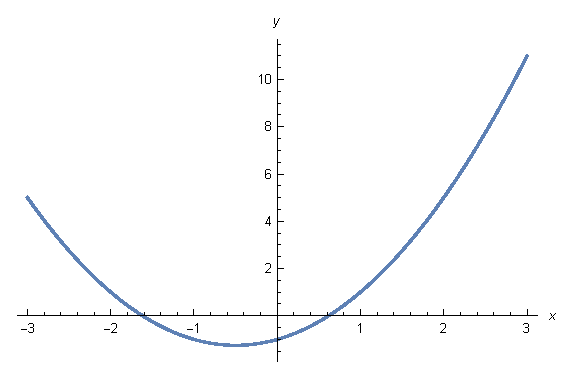
\includegraphics[width=0.5\textwidth]{image/2.1.5function1.eps}
  \label{img:2.1.5function1}
\end{figure}

\begin{example}
  函数$f(x)=x^3-x^2+x-3$的部分图像如下:
\end{example}

\begin{figure}[h]
  \centering
  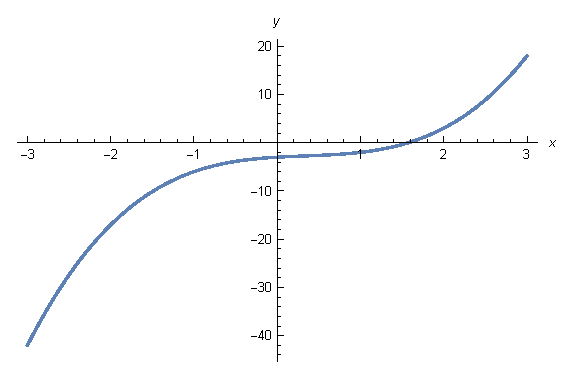
\includegraphics[width=0.5\textwidth]{image/2.1.5function2.eps}
  \label{img:2.1.5function2}
\end{figure}

\begin{example}{下取整函数}
  记$\lfloor x\rfloor $为小于或等于$x$的最大整数,则下取整函数可记作$f(x)=\lfloor x\rfloor$.图像如下:
\end{example}

\begin{figure}[h]
  \centering
  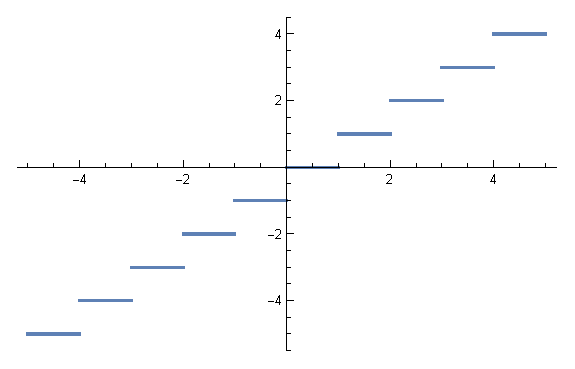
\includegraphics[width=0.5\textwidth]{image/2.1.5function5.eps}
  \label{img:2.1.5function5}
\end{figure}

解题时若恰当运用函数图像,有事半功倍的效果。

接下来我们来看函数图像的变换。以下设$p(x,y)$为\textcolor{blue}{变换后}函数图像上任意一点,$P'(x',y')$为\textcolor{blue}{原函数}图像上对应于点$P$的一点。

\subsubsection{平移变换}

将$y=f(x)$(这是原函数,这里的$x$和下面的$x$并不一样)的图像向左平移$h$个单位长度,则有
$\begin{cases}
  x=x'-h
  \\y=y'
\end{cases}$,也就是
$\begin{cases}
  x'=x+h
  \\y'=y
\end{cases}$,
由于$y'=f(x')$,把$x',y'$代回去,可知变换后的函数图像为$y=f(x+h)$的图像。

同理可得:

\begin{enumerate}
  \item 将$y=f(x)$的图像向右平移$h$个单位长度得到$y=f(x-h)$的图像;
  \item 将$y=f(x)$的图像向下平移$h$个单位长度得到$y=f(x)-h$的图像;
  \item 将$y=f(x)$的图像向上平移$h$个单位长度得到$y=f(x)+h$的图像。
\end{enumerate}

\begin{exercise}
  证明上述规律。
\end{exercise}

\subsubsection{伸缩变换}

\begin{enumerate}
  \item 横向伸缩:将函数$y=f(x)$的图像上所有点的横坐标变为原来的$\omega(\omega\neq 0)$倍后得到函数$y=f(\dfrac{x}{\omega})$的图像。
  \item 纵向伸缩:将函数$y=f(x)$的图像上所有点的纵坐标变为原来的$\omega$倍后得到函数$y=\omega f(x)$的图像。
\end{enumerate}

证明方法和前面类似。

\subsubsection{翻折变换}

\begin{enumerate}
  \item 下翻上:将函数$y=f(x)$在$x$轴下方这一部分的图像沿着$x$轴翻折,即得$\left| f(x)\right|$的图像;
  \item 右翻左:将函数$y=f(x)$在$y$轴右侧这一部分的图像沿着$y$轴翻折,即得$f(\left| x\right|)$的图像。
\end{enumerate}

\subsubsection{对称变换}

\begin{enumerate}
  \item 函数$y=f(x)$的图像与函数$y=f(-x)$的图像关于$y$轴对称;
  \item 函数$y=f(x)$的图像与函数$y=-f(x)$的图像关于$x$轴对称;
  \item 函数$y=f(x)$的图像与函数$y=-f(-x)$的图像关于原点对称。
\end{enumerate}

\begin{example}
  作出函数$y=\left| x^2+2x-2\right|$的图像。
\end{example}

\begin{solution}
  如图所示。
\end{solution}

\begin{figure}[h]
  \centering
  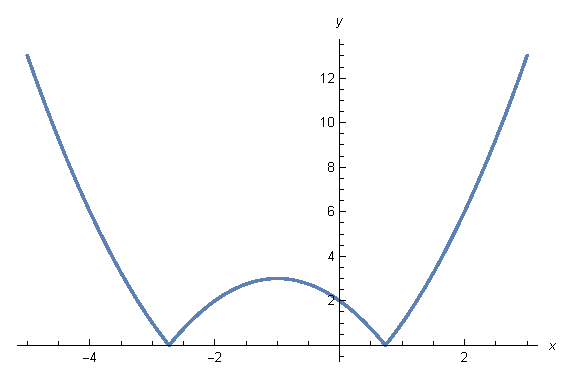
\includegraphics[width=0.5\textwidth]{image/2.1.5function3.eps}
  \label{img:2.1.5function3}
\end{figure}

\begin{example}
  作出函数$f(x)=\dfrac{3x-7}{x-2}$的图像。
\end{example}

\begin{spacing}{1.8}
  
\end{spacing}
\begin{solution}
  \begin{spacing}{1.8}
    $f(x)=\dfrac{3x-7}{x-2}=3-\dfrac{1}{x-2}$,可见$f(x)$的图像是由$g(x)=-\dfrac{1}{x}$的图像向右平移2个单位长度,再向上平移$3$个单位长度得到。如图所示。
  \end{spacing}
\end{solution}

\begin{figure}[h]
  \centering
  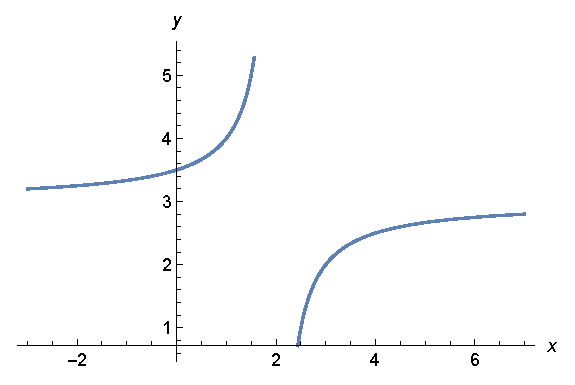
\includegraphics[width=0.5\textwidth]{image/2.1.5function4.eps}
  \label{img:2.1.5function4}
\end{figure}

\subsection{使用工具软件绘制函数图像}

\subsubsection{Geogebra}

Geogebra是一款免费的数学工具软件,主要包含图形计算器、几何、3D计算器和CAS计算器四个模块,我个人最常使用的是图形计算器(几何图形也可以用这个定位)。官网是\href{https://www.geogebra.org/}{https://www.geogebra.org/},在这里既可以下载Geogebra计算器的APP(\href{https://www.geogebra.org/download}{https://www.geogebra.org/download}),也可以点击“打开计算器”直接打开在线版使用。

我们以Windows版的Geogebra为例,作函数$f(x)=x^3+x^2+1$的图像关于原点对称。

下载完安装包后直接打开,等待Geogebra自动安装。安装完后启动Geogebra,你应该会看到类似于\ref{img:geogebra1}的界面:

\begin{figure}[h]
  \centering
  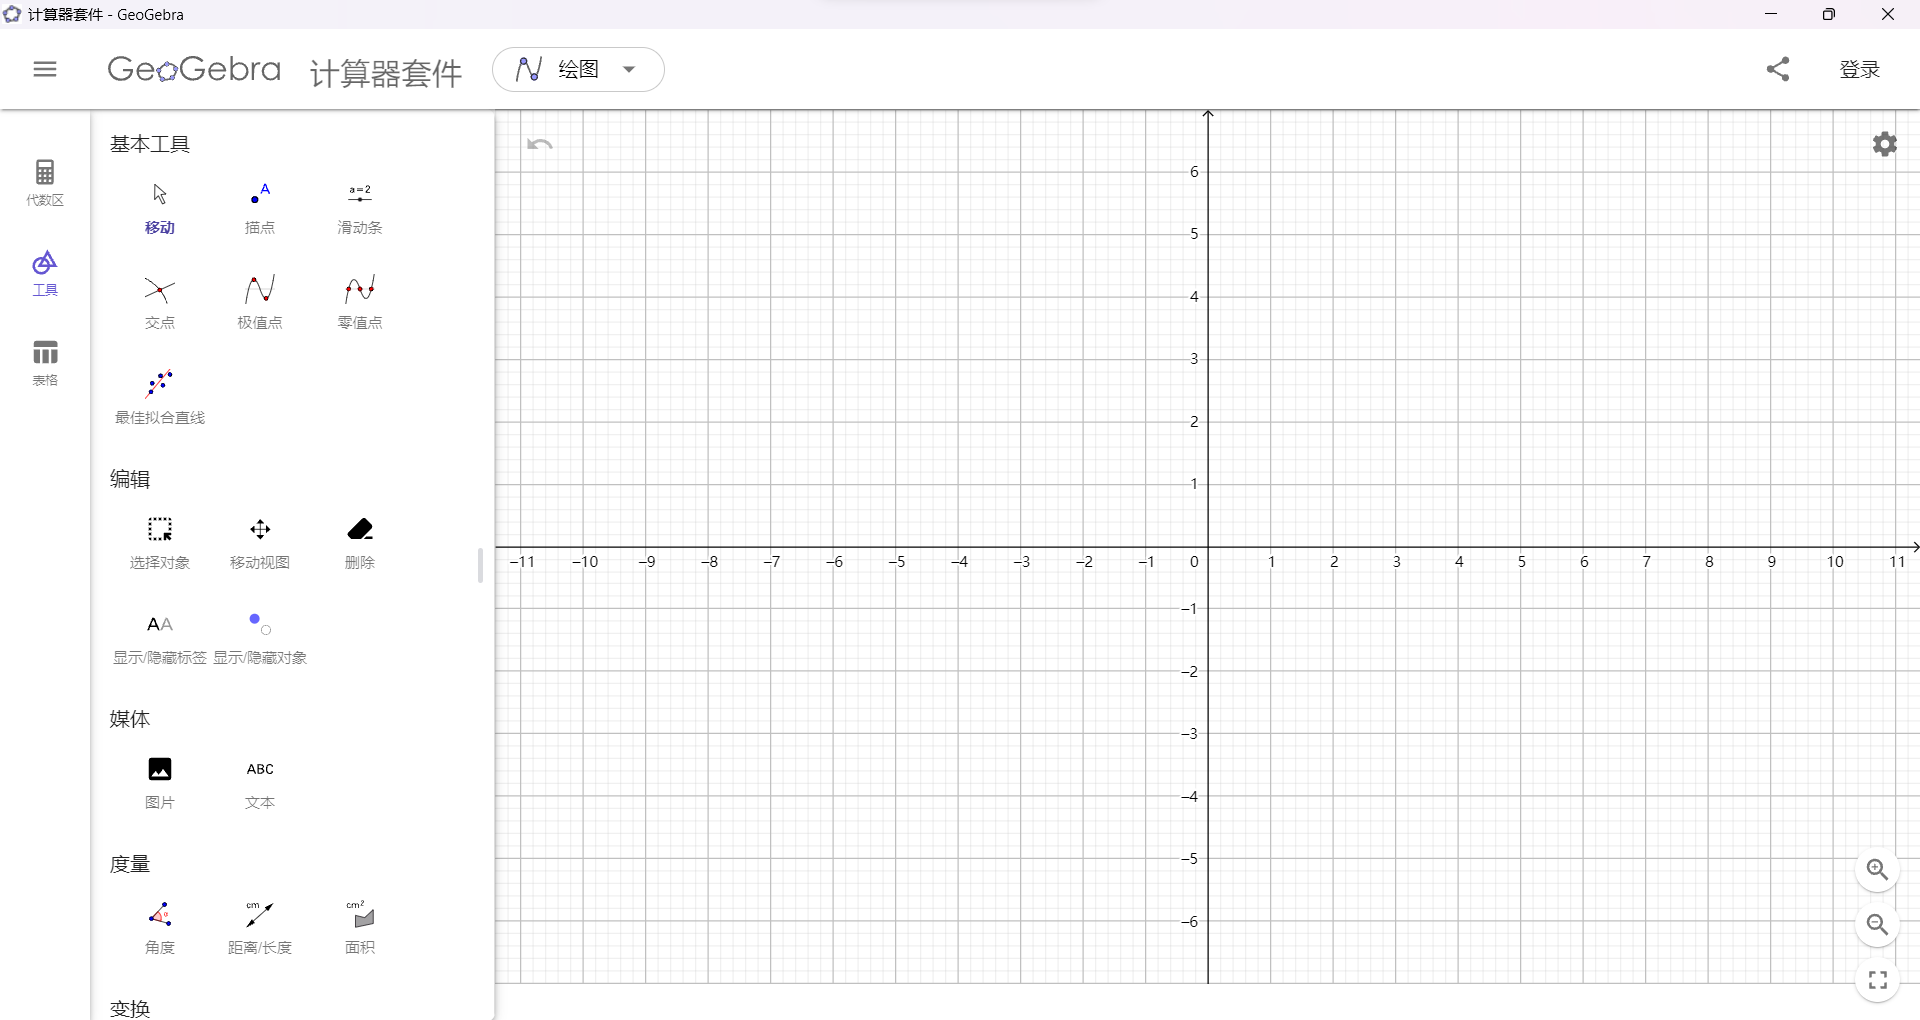
\includegraphics[width=0.7\textwidth]{image/geogebra1.png}
  \caption{Geogebra启动界面}
  \label{img:geogebra1}
\end{figure}

\begin{remark}
  如果你通过上面给的下载链接进入后直接点击“下载”,默认下载的是Geogebra 6。
\end{remark}

\hspace*{\fill}

点击左边的“代数区”,再点击左下角的键盘图标唤出键盘,效果如\ref{img:geogebra2}所示。

\begin{figure}[h]
  \centering
  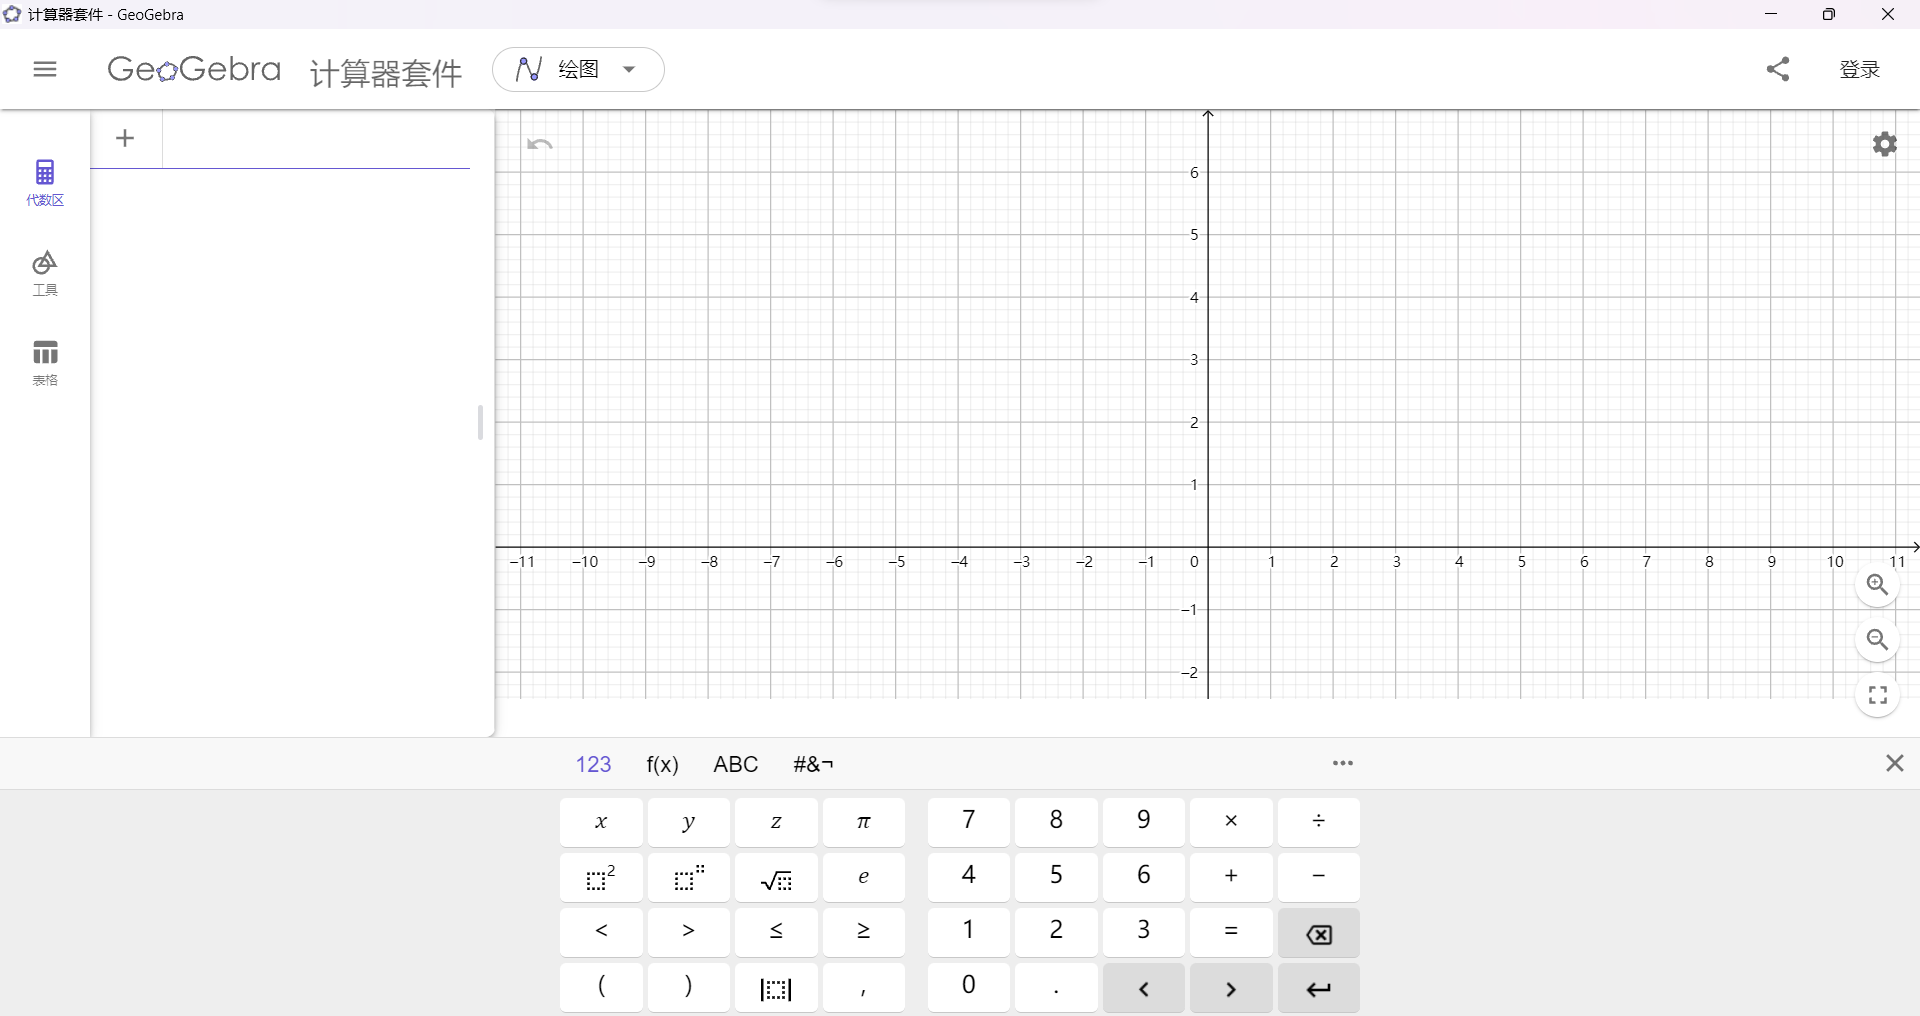
\includegraphics[width=0.7\textwidth]{image/geogebra2.png}
  \caption{打开代数区}
  \label{img:geogebra2}
\end{figure}

点击左上角有“输入”二字的输入框,然后按\ref{img:geogebra3}所示数字顺序操作。

\begin{figure}[h]
  \centering
  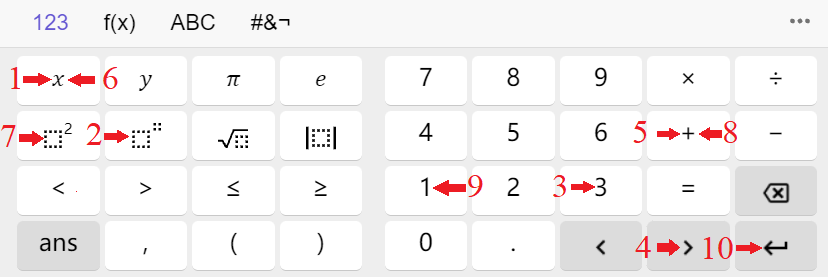
\includegraphics[width=0.5\textwidth]{image/geogebra3.png}
  \caption{操作顺序}
  \label{img:geogebra3}
\end{figure}

结果应该如\ref{img:geogebra4}所示。你可以通过右侧红圈处的两个按钮放大或缩小图像。更多的功能你可以自行探索。需要注意的是,保存时若弹出一个空白窗口,直接关掉即可。这个登录界面是连接不到的。

\begin{figure}[h]
  \centering
  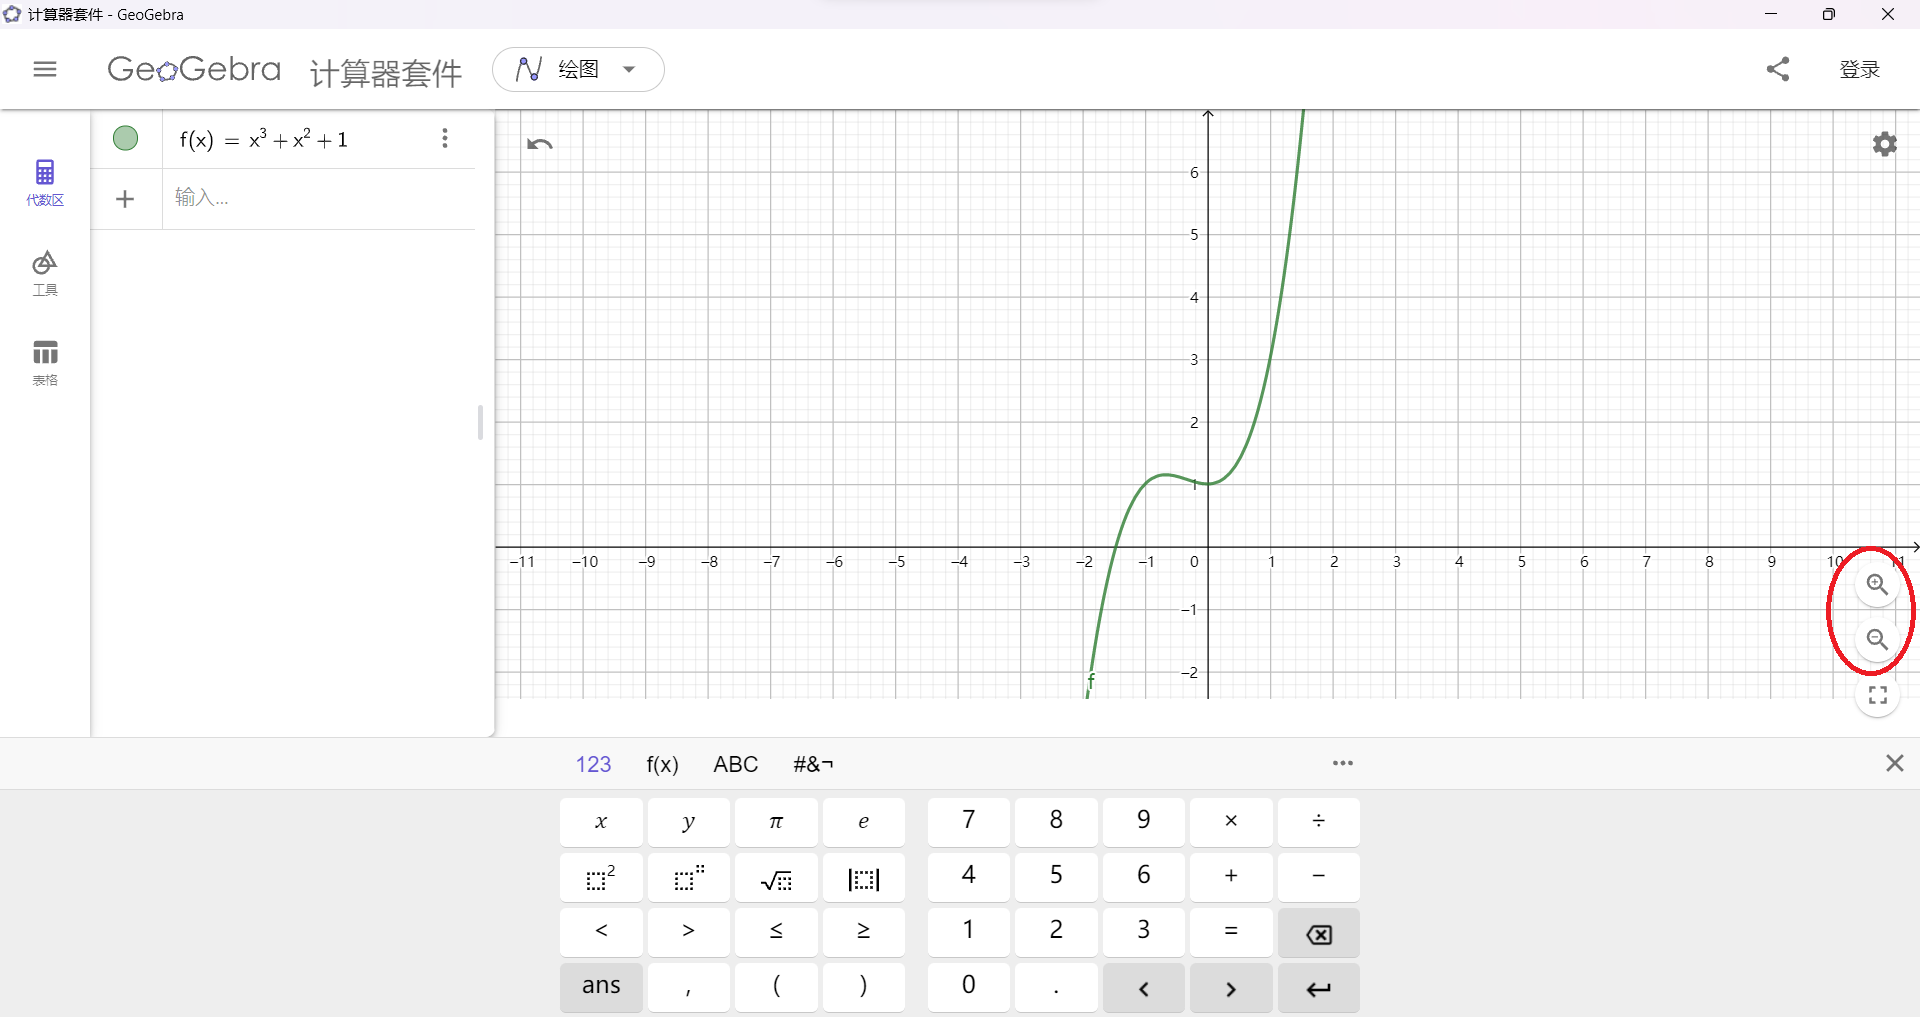
\includegraphics[width=0.7\textwidth]{image/geogebra4.png}
  \caption{绘制出的函数图像}
  \label{img:geogebra4}
\end{figure}

\subsubsection{Mathematica}

Mathematica是一款极为强大的\underline{专业}数学工具软件。基本上啥都能干。

(官网:\href{https://www.wolfram.com/mathematica/}{https://www.wolfram.com/mathematica/})

当然,这是个付费软件,而且并不方便购买。官网有提供试用,但我对此不太了解。若你有条件激活Mathematica,你可以体验一下它的强大功能;若没有条件,下文权当放松一下。

在此我们展示一下它的绘制函数图像功能。

\begin{figure}[h]
  \centering
  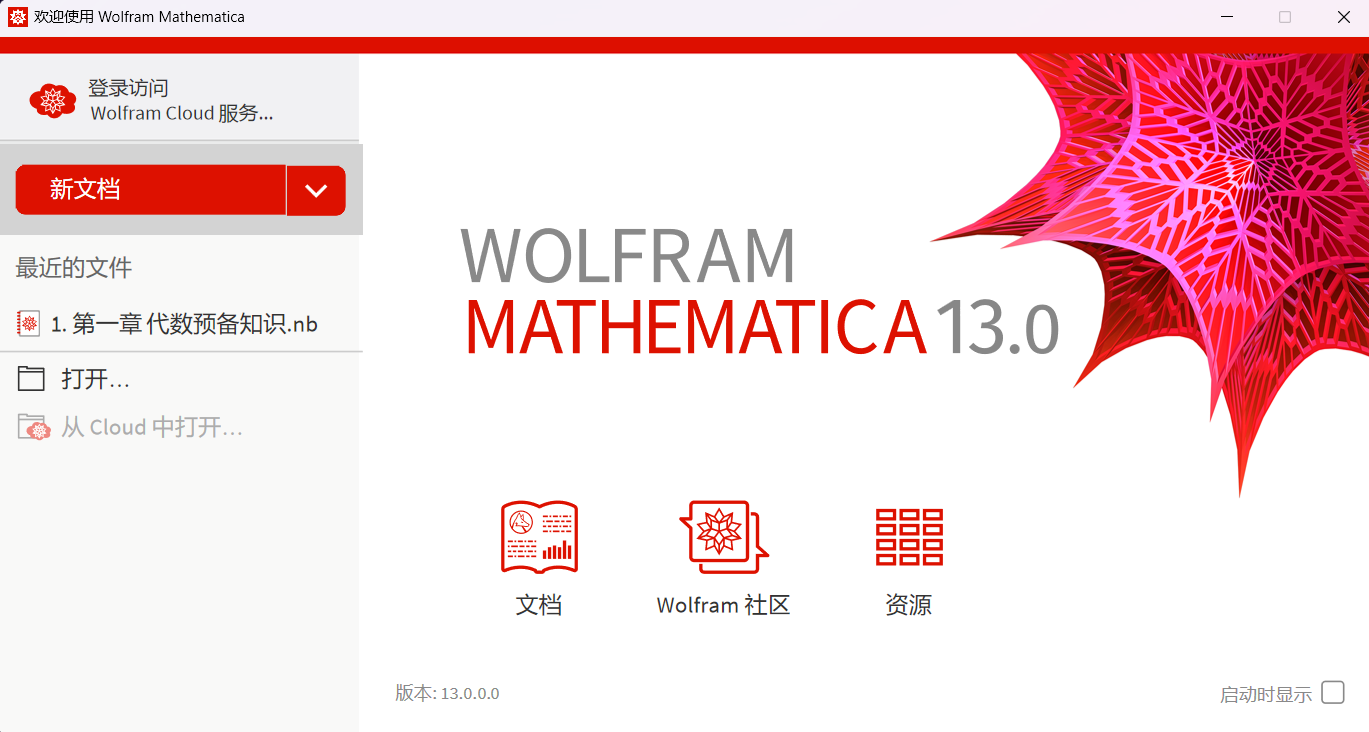
\includegraphics[width=0.6\textwidth]{image/mathematica1.png}
  \caption{Mathematica启动界面}
  \label{img:mathematica1}
\end{figure}

点击“新文档”新建一个文件。输入“Plot$\left[\text{x}^{\land}3+\text{x}^{\land}2+1,\{\text{x},-5,5\}\right]$”,按下\textcolor{blue}{Shift键+Enter键}即可。如图\ref{img:mathematica2}所示。

\begin{figure}[h]
  \centering
  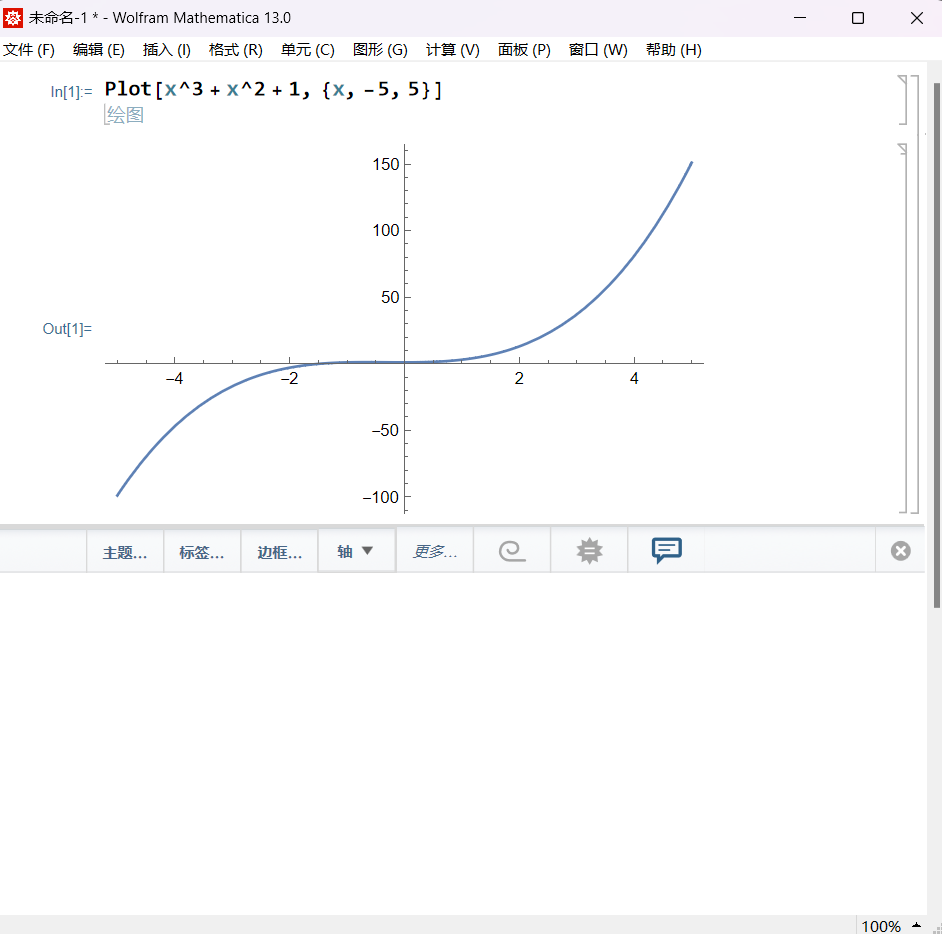
\includegraphics[width=0.6\textwidth]{image/mathematica2.png}
  \caption{Mathematica绘制函数图像}
  \label{img:mathematica2}
\end{figure}

\begin{remark}
  Plot是绘制函数图像的命令。格式为Plot[$f,\left\{x,x_{min},x_{max}\right\}$],表示绘制函数$f$的图像,其中$x$的取值范围为$x_{min}$到$x_{max}$.
\end{remark}

使用Mathematica需要善用帮助文档(\href{https://reference.wolfram.com/language/}{https://reference.wolfram.com/language/})。

在学习数学的过程中,工具软件可以帮我们减少许多麻烦。当然,不可完全依赖工具软件,将其作为辅助是一个不错的选择。当然,AI也同样是好帮手,可惜目前AI在本书的知识领域内容易出错(2024.8.28)。

\subsection{习题}

\begin{exercise}\label{2017RJB.P94.8.changed}
  已知函数$f(x+2)=3x-7$,求$f(1),f(x)$.
\end{exercise}

\begin{exercise}
  设函数$f(x)=x^2-7,g(x)=4x+8$,求$f(g(x)),g(f(x))$.
\end{exercise}

\begin{exercise}
  作出下列函数的大致图像:
\end{exercise}

\begin{spacing}{1.8}
  \begin{enumerate}
    \item $f(x)=\dfrac12 x^2-x+2$;
    \item $f(x)=x^3-2x+7$;
    \item $f(x)=\dfrac{1}{10}x^4-x^2-5$;
    \item $f(x)=\dfrac{x-1}{2x+1}$;
    \item $f(x)=\sqrt{x-1}$;
    \item $f(x)=\left|x\right|^2+\left|x\right|+2$;
    \item $f(x)=\dfrac{1-\left|x\right|}{\left|1-x\right|}$;
    \item $f(x)=1+\sqrt{x^{2}+2x}$.
  \end{enumerate}
\end{spacing}

\begin{exercise}\label{BJSZ.Algebra1.P58-59.changed}
  下列各题中,函数$f_1(x)$的图像经过怎样的变换可得到$f_2(x)$的图像?
\end{exercise}

\begin{spacing}{1.7}
  \begin{enumerate}
    \item $f_{1}(x)=2(x+2)^{2}, f_{2}(x)=2(x-2)^{2}+1$;
    \item $f_{1}(x)=\dfrac{1}{x}, f_{2}(x)=\dfrac{1}{2x+3}$;
    \item $f_{1}\left(x\right)=\left(x-1\right)^{2}-3,\quad f_{2}\left(x\right)=\left|\left(x-1\right)^{2}-3\right|$;
    \item $f_{1}(x)=(x-1)^{2}-3,f_{2}(x)=(|x|-1)^{2}-3$.
  \end{enumerate}
\end{spacing}

\begin{exercise}
  定义域为$\mathbb{R}$的函数$f(x)$满足以下条件,分别写出对应条件下$f(x)$的一条对称轴:
\end{exercise}

\begin{enumerate}
  \item $f(1-x)=f(1+x)$;
  \item $f(x-1)=f(2-x)$;
  \item $f(b+x)=f(c-x)$.
\end{enumerate}

\begin{exercise}
  定义域为$\mathbb{R}$的函数$f(x)$满足以下条件,分别写出对应条件下$f(x)$关于哪一点对称:
\end{exercise}

\begin{enumerate}
  \item $f(2-x)=-f(2+x)$;
  \item $f(2-x)=-f(1+x)$;
  \item $f(a-x)+f(c+x)=0$;
  \item $f(a-x)+f(c+x)=2b$.
\end{enumerate}

\begin{exercise}
  已知函数$f(x)$,若存在$x\in\mathbb{R}$使得$f(x)=x$,则称$x$为$f(x)$的不动点。
\end{exercise}

\begin{enumerate}
  \item 求证:$f(x)$的不动点也是$f(f(x))$的不动点;
  \item 求证:若$f(f(x))$有唯一的不动点,则$f(x)$也有唯一的不动点。
\end{enumerate}

\begin{exercise}\label{ASJC_G1_P22.5}
  求证:对任意的实数$p$,抛物线$y=2x^2-px+4p+1$恒过一定点。
\end{exercise}

\begin{exercise}
  设$f_n(x)=\underbrace{f\{f[\cdots f(x)]\}}_{n\text{次}}$,若$f(x)=\dfrac{x}{\sqrt{1+x^2}}$,求$f_n(x)$.
\end{exercise}

\begin{exercise}
  设二次函数$f(x)=ax^{2}+bx+c(a>0)$,方程$f(x)-x=0$的两根$x_1,x_2$满足$0<x_1<x_2<\dfrac1a$.
\end{exercise}

\begin{enumerate}
  \item 当$x\in(0,x_1)$时,求证:$x<f(x)<x_1$;
  \item 设函数$f(x)$的图像关于$x=x_0$对称,求证:$x_0<\dfrac{x_1}{2}$.
\end{enumerate}

\begin{remark}
  这是1997年全国高考数学试题(理工农医类)的压轴题,有相当的难度。
\end{remark}

\section{函数的基本性质}

\subsection{函数的单调性}

\subsection{函数的奇偶性}

\subsection{函数的周期性}

\end{document}